% Options for packages loaded elsewhere
\PassOptionsToPackage{unicode}{hyperref}
\PassOptionsToPackage{hyphens}{url}
%
\documentclass[
  11pt,
  english,
  man,floatsintext]{apa6}
\title{What we do (not) know about the mechanisms underlying adaptive speech perception: A computational review}
\author{Xin Xie\textsuperscript{1,2}, T. Florian Jaeger\textsuperscript{2,3}, \& Chigusa Kurumada\textsuperscript{2}}
\date{June 28, 2022}

\usepackage{amsmath,amssymb}
\usepackage{lmodern}
\usepackage{iftex}
\ifPDFTeX
  \usepackage[T1]{fontenc}
  \usepackage[utf8]{inputenc}
  \usepackage{textcomp} % provide euro and other symbols
\else % if luatex or xetex
  \usepackage{unicode-math}
  \defaultfontfeatures{Scale=MatchLowercase}
  \defaultfontfeatures[\rmfamily]{Ligatures=TeX,Scale=1}
\fi
% Use upquote if available, for straight quotes in verbatim environments
\IfFileExists{upquote.sty}{\usepackage{upquote}}{}
\IfFileExists{microtype.sty}{% use microtype if available
  \usepackage[]{microtype}
  \UseMicrotypeSet[protrusion]{basicmath} % disable protrusion for tt fonts
}{}
\makeatletter
\@ifundefined{KOMAClassName}{% if non-KOMA class
  \IfFileExists{parskip.sty}{%
    \usepackage{parskip}
  }{% else
    \setlength{\parindent}{0pt}
    \setlength{\parskip}{6pt plus 2pt minus 1pt}}
}{% if KOMA class
  \KOMAoptions{parskip=half}}
\makeatother
\usepackage{xcolor}
\IfFileExists{xurl.sty}{\usepackage{xurl}}{} % add URL line breaks if available
\IfFileExists{bookmark.sty}{\usepackage{bookmark}}{\usepackage{hyperref}}
\hypersetup{
  pdftitle={What we do (not) know about the mechanisms underlying adaptive speech perception: A computational review},
  pdfauthor={Xin Xie1,2, T. Florian Jaeger2,3, \& Chigusa Kurumada2},
  pdflang={en-EN},
  pdfkeywords={speech perception; computational model; accent adaptation; perceptual recalibration},
  hidelinks,
  pdfcreator={LaTeX via pandoc}}
\urlstyle{same} % disable monospaced font for URLs
\usepackage{graphicx}
\makeatletter
\def\maxwidth{\ifdim\Gin@nat@width>\linewidth\linewidth\else\Gin@nat@width\fi}
\def\maxheight{\ifdim\Gin@nat@height>\textheight\textheight\else\Gin@nat@height\fi}
\makeatother
% Scale images if necessary, so that they will not overflow the page
% margins by default, and it is still possible to overwrite the defaults
% using explicit options in \includegraphics[width, height, ...]{}
\setkeys{Gin}{width=\maxwidth,height=\maxheight,keepaspectratio}
% Set default figure placement to htbp
\makeatletter
\def\fps@figure{htbp}
\makeatother
\setlength{\emergencystretch}{3em} % prevent overfull lines
\providecommand{\tightlist}{%
  \setlength{\itemsep}{0pt}\setlength{\parskip}{0pt}}
\setcounter{secnumdepth}{5}
% Make \paragraph and \subparagraph free-standing
\ifx\paragraph\undefined\else
  \let\oldparagraph\paragraph
  \renewcommand{\paragraph}[1]{\oldparagraph{#1}\mbox{}}
\fi
\ifx\subparagraph\undefined\else
  \let\oldsubparagraph\subparagraph
  \renewcommand{\subparagraph}[1]{\oldsubparagraph{#1}\mbox{}}
\fi
\newlength{\cslhangindent}
\setlength{\cslhangindent}{1.5em}
\newlength{\csllabelwidth}
\setlength{\csllabelwidth}{3em}
\newlength{\cslentryspacingunit} % times entry-spacing
\setlength{\cslentryspacingunit}{\parskip}
\newenvironment{CSLReferences}[2] % #1 hanging-ident, #2 entry spacing
 {% don't indent paragraphs
  \setlength{\parindent}{0pt}
  % turn on hanging indent if param 1 is 1
  \ifodd #1
  \let\oldpar\par
  \def\par{\hangindent=\cslhangindent\oldpar}
  \fi
  % set entry spacing
  \setlength{\parskip}{#2\cslentryspacingunit}
 }%
 {}
\usepackage{calc}
\newcommand{\CSLBlock}[1]{#1\hfill\break}
\newcommand{\CSLLeftMargin}[1]{\parbox[t]{\csllabelwidth}{#1}}
\newcommand{\CSLRightInline}[1]{\parbox[t]{\linewidth - \csllabelwidth}{#1}\break}
\newcommand{\CSLIndent}[1]{\hspace{\cslhangindent}#1}
\usepackage{fontspec}

%% Pandoc can only set 10, 11, 12 pt
%% uncomment below to set fontsize
%\usepackage[fontsize=13pt]{scrextend}

%\setmainfont{Calibri} % Set main font for latin characters

\setlength{\parskip}{0.15cm} % Set space between paragraphs
%\linespread{1.2}\selectfont % Set line height
%\usepackage[doublespacing]{setspace} % Use double space without changing footnotes line height

%% Special font for IPA
%% Make sure "Doulos SIL" is installed on your computer
%% For other typefaces supporting IPA symbols, see
%% https://en.wikipedia.org/wiki/International_Phonetic_Alphabet#Typefaces
\newfontfamily\ipa{Doulos SIL} % Font for IPA symbols
\DeclareTextFontCommand{\ipatext}{\ipa}



%%%         Section for CJK Characters                   %%%
%%%   You may want to uncomment the code below if        %%%
%%%   you're writing this document with CJK characters   %%%

%\usepackage{xeCJK}  % Uncomment for using CJK characters
%% Set main font for CJK characters
%% Make sure your system has the font set
%\setCJKmainfont[
%	BoldFont={HanWangHeiHeavy}  % Set font for CJK boldface
%    ]{標楷體}    % Set font for normal CJK
%% Some Traditional Chinese fonts: AR PL KaitiM Big5, PingFang TC, Noto Sans CJK TC
%\XeTeXlinebreaklocale "zh"
%\XeTeXlinebreakskip = 0pt plus 1pt
% Manuscript styling
\usepackage{upgreek}
\captionsetup{font=singlespacing,justification=justified}

% Table formatting
\usepackage{longtable}
\usepackage{lscape}
% \usepackage[counterclockwise]{rotating}   % Landscape page setup for large tables
\usepackage{multirow}		% Table styling
\usepackage{tabularx}		% Control Column width
\usepackage[flushleft]{threeparttable}	% Allows for three part tables with a specified notes section
\usepackage{threeparttablex}            % Lets threeparttable work with longtable

% Create new environments so endfloat can handle them
% \newenvironment{ltable}
%   {\begin{landscape}\centering\begin{threeparttable}}
%   {\end{threeparttable}\end{landscape}}
\newenvironment{lltable}{\begin{landscape}\centering\begin{ThreePartTable}}{\end{ThreePartTable}\end{landscape}}

% Enables adjusting longtable caption width to table width
% Solution found at http://golatex.de/longtable-mit-caption-so-breit-wie-die-tabelle-t15767.html
\makeatletter
\newcommand\LastLTentrywidth{1em}
\newlength\longtablewidth
\setlength{\longtablewidth}{1in}
\newcommand{\getlongtablewidth}{\begingroup \ifcsname LT@\roman{LT@tables}\endcsname \global\longtablewidth=0pt \renewcommand{\LT@entry}[2]{\global\advance\longtablewidth by ##2\relax\gdef\LastLTentrywidth{##2}}\@nameuse{LT@\roman{LT@tables}} \fi \endgroup}

% \setlength{\parindent}{0.5in}
% \setlength{\parskip}{0pt plus 0pt minus 0pt}

% \usepackage{etoolbox}
\makeatletter
\patchcmd{\HyOrg@maketitle}
  {\section{\normalfont\normalsize\abstractname}}
  {\section*{\normalfont\normalsize\abstractname}}
  {}{\typeout{Failed to patch abstract.}}
\patchcmd{\HyOrg@maketitle}
  {\section{\protect\normalfont{\@title}}}
  {\section*{\protect\normalfont{\@title}}}
  {}{\typeout{Failed to patch title.}}
\makeatother
\shorttitle{Exposure effects in speech perception}
\keywords{speech perception; computational model; accent adaptation; perceptual recalibration\newline\indent Word count: X}
\usepackage{lineno}

\linenumbers
\usepackage{csquotes}
\usepackage{animate}
\usepackage{amsmath}
\usepackage{tikz}
\usetikzlibrary{bayesnet}
\usepackage{booktabs}
\usepackage{siunitx}
\usepackage{soul}
\usepackage{tabto}
\usepackage{xcolor}
\usepackage{placeins}
\setstcolor{red}
\usepackage{sectsty}
\sectionfont{\color{black}}
\subsectionfont{\color{black}}
\subsubsectionfont{\color{black}}
\usepackage{setspace}\doublespacing
\usepackage{subfig}
\ifXeTeX
  % Load polyglossia as late as possible: uses bidi with RTL langages (e.g. Hebrew, Arabic)
  \usepackage{polyglossia}
  \setmainlanguage[]{english}
\else
  \usepackage[main=english]{babel}
% get rid of language-specific shorthands (see #6817):
\let\LanguageShortHands\languageshorthands
\def\languageshorthands#1{}
\fi
\ifLuaTeX
  \usepackage{selnolig}  % disable illegal ligatures
\fi


\authornote{

We are grateful to \#\#\# ommitted for review \#\#\#

Correspondence concerning this article should be addressed to Xin Xie, 3151 Social Science Plaza B, University of California, Irvine CA 92697--5100. E-mail: \href{mailto:xie14@uci.edu}{\nolinkurl{xie14@uci.edu}}

}

\affiliation{\vspace{0.5cm}\textsuperscript{1} Language Science, University of California, Irvine\\\textsuperscript{2} Brain and Cognitive Sciences, University of Rochester\\\textsuperscript{3} Computer Science, University of Rochester}

\abstract{
Speech from unfamiliar talkers can be difficult to comprehend initially. These difficulties tend to dissipate with exposure, sometimes within minutes or less. Adaptivity in response to unfamiliar input is now considered a fundamental property of speech perception, and research over the past two decades has made substantial progress in identifying its characteristics. The \emph{mechanisms} underlying adaptive speech perception, however, remain unknown. Past work has attributed facilitatory effects of exposure to any one of three qualitatively different hypothesized mechanisms: (1) low-level, pre-linguistic, signal normalization, (2) changes in/selection of linguistic representations, or (3) changes in post-perceptual decision-making. Direct comparisons of these hypotheses have been lacking, in part for a lack of sufficiently concrete (testable) theories and models. We describe a general computational framework that---for the first time---implements all three major mechanisms through which recent exposure can come to affect subsequent perception. We demonstrate how the framework can be used to derive predictions for experiments on perception from the acoustic properties of the stimuli. Using this approach, we find that the signature results of common experimental paradigms do not distingish between the three mechanisms. This highlights the need for a change in research practices, so that future experiments provide more informative results. We recommend specific changes to experimental paradigms, data analysis, and data sharing to overcome this empirical indeterminacy. All data and code for this study are shared via OSF, including the R markdown document that this article is generated from, and an R library that implements the models we present.
}



\begin{document}
\maketitle

\hypertarget{introduction}{%
\section{Introduction}\label{introduction}}

How human listeners understand speech is a central question in cognitive science. The computational complexity of spoken language understanding becomes most apparent when a talker's pronunciations---and thus the mapping of acoustic input to linguistic categories and meaning---strongly deviate from listeners' expectations. This might occur, for example, when listening to talkers with unfamiliar regional or non-native accents, or patients with apraxia or dysarthria. The same fundamental challenge is, however, present even during seemingly effortless comprehension: even among talkers who share similar language backgrounds, the mapping between the acoustic input and linguistic categories can vary substantially between talkers due to both physiology (e.g., vocal tract size and shape) and socio-cultural factors (e.g., social identity and language background). As a consequence, one talker's pronunciation of, say, the sound category {[}s{]} (as in \emph{sip}) can be acoustically more similar to another talker's production of {[}\ipatext{ʃ}{]} (as in \emph{ship}, Newman et al., \protect\hyperlink{ref-newman2001}{2001}). How we manage to typically understand each other despite such cross-talker differences has remained one of the perennial puzzles in research on speech perception (where it is known as part of the infamous \emph{lack of invariance} problem, \protect\hyperlink{ref-liberman1967}{Liberman, Cooper, Shankweiler, \& Studdert-Kennedy, 1967}). In the present project, we outline a general computational framework that can help address this question, by---for the first time---implementing competing hypotheses about the mechanisms underlying listeners' ability to accommodate cross-talker variability. Our goal is to demonstrate how the framework works, what it offers, and why a computational approach like this is needed. We use the framework to show that we know much \emph{less} about the perceptual mechanisms underlying speech perception than is often assumed. We then discuss how to design more decisive behavioral experiments that are more suited to distinguish between competing hypotheses about these mechanisms.

Research over the past decades has identified adaptive changes in speech perception to be a key component in listeners' ability to overcome cross-talker differences. Although speech perception can initially be slower and/or less accurate when listeners encounter an unfamiliar talkers with unexpected pronunciations, these processing difficulties tend to reduce with exposure (e.g., \protect\hyperlink{ref-bradlow-bent2008}{Bradlow \& Bent, 2008}; \protect\hyperlink{ref-nygaard1994}{Nygaard, Sommers, \& Pisoni, 1994}; \protect\hyperlink{ref-Perrachione2016}{Tyler K. Perrachione et al., 2016}; \protect\hyperlink{ref-sidaras2009}{Sidaras, Alexander, \& Nygaard, 2009}; \protect\hyperlink{ref-wade2007}{Wade, Jongman, \& Sereno, 2007}; \protect\hyperlink{ref-weil2001a}{Weil, 2001}; \protect\hyperlink{ref-xie2021jep}{Xie, Liu, \& Jaeger, 2021}). Remarkably, substantial improvements can occur within minutes or less (\protect\hyperlink{ref-clarke-garrett2004}{Clarke \& Garrett, 2004}; \protect\hyperlink{ref-munro-derwing1995}{Munro \& Derwing, 1995}; \protect\hyperlink{ref-xie2018jasa}{Xie et al., 2018}). Even a context as brief as a single utterance can be sufficient to change perception and segmentation of ambiguous speech (e.g., categorizing a Dutch ambiguous /m?t/ embedded in an utterance with fast or slow speech as either {``mat''} or {``maat''} Bosker et al., \protect\hyperlink{ref-bosker2017}{2017}). (see also \protect\hyperlink{ref-kluender1988}{Kluender, Diehl, \& Wright, 1988}; \protect\hyperlink{ref-newman-sawusch1996}{Newman \& Sawusch, 1996}; \protect\hyperlink{ref-sawusch-newman2000}{Sawusch \& Newman, 2000}; \protect\hyperlink{ref-sjerps2011}{Sjerps, Mitterer, \& McQueen, 2011a}). Multiple neurobiological systems have been proposed to support these rapid changes (e.g., \protect\hyperlink{ref-adank2015}{\textbf{adank2015?}}). They range from the primary auditory cortex (e.g., Heschl's gyrus, \protect\hyperlink{ref-Perrachione2007}{T. K. Perrachione \& Wong, 2007}) to those that respond to acoustic-phonetic features in speech (e.g., superior temporal gyrus, \protect\hyperlink{ref-Yi2019}{Yi, Leonard, \& Chang, 2019}). Heterogeneous networks come together to recognize a voice/talker (\protect\hyperlink{ref-luthra2020b}{Luthra, 2020}), attend selectively to a given talker's speech (\protect\hyperlink{ref-wong2004}{Wong, Nusbaum, \& Small, 2004}), and correct prediction errors when there is a discrepancy between a predicted vs.~an actual input (e.g., \protect\hyperlink{ref-guediche2015evidence}{Guediche, Holt, Laurent, Lim, \& Fiez, 2015}).

In short, listeners' ability to adapt based on recent input is now considered a central part of human speech perception. Explaining how it can be done has motivated major theories of speech perception and comprehension.\footnote{Additional lines of work have investigated exposure to synthesized, vocoded, or otherwise distorted speech (e.g., \protect\hyperlink{ref-adank2009}{Adank, Evans, Stuart-Smith, \& Scott, 2009}; \protect\hyperlink{ref-davis2005}{Davis, Johnsrude, Hervais-Adelman, Taylor, \& McGettigan, 2005}; \protect\hyperlink{ref-fenn2003}{Fenn, Nusbaum, \& Margoliash, 2003}; \protect\hyperlink{ref-mattys2012}{Mattys, Davis, Bradlow, \& Scott, 2012}) or have used distributional learning paradigms (e.g., \protect\hyperlink{ref-clare2019}{Clare, 2019}; \protect\hyperlink{ref-clayards2008}{Clayards, Tanenhaus, Aslin, \& Jacobs, 2008}; \protect\hyperlink{ref-idemaru-holt2011}{Idemaru \& Holt, 2011}; \protect\hyperlink{ref-maye2008}{Maye, Aslin, \& Tanenhaus, 2008}; \protect\hyperlink{ref-schertz2013}{Schertz, 2013}; \protect\hyperlink{ref-theodore-monto2019}{Theodore \& Monto, 2019}; \protect\hyperlink{ref-wade2007}{Wade et al., 2007}). In the general discussion, we return to distributional learning paradigms, which we believe to hold particular promise in addressing the issues we identify below.} Despite these substantial advances, however, mechanistic origins of the adaptivity are not yet well understood. Different explanations continue to coexist across different lines of work, each with qualitatively different implications for the cognitive and neural accounts of how---through what mechanisms---exposure comes to facilitate comprehension (for reviews, see \protect\hyperlink{ref-baeseberk2020}{Baese-Berk, McLaughlin, \& McGowan, 2020}; \protect\hyperlink{ref-johnson-sjerps2021}{Johnson \& Sjerps, 2021}; \protect\hyperlink{ref-quam-creel2021}{Quam \& Creel, 2021}; \protect\hyperlink{ref-samuel-kraljic2009}{Samuel \& Kraljic, 2009}; \protect\hyperlink{ref-stilp2020}{Stilp, 2020}; \protect\hyperlink{ref-weatherholtz-jaeger2016}{Weatherholtz \& Jaeger, 2016}).

While different in important details, existing theories in speech perception share general assumptions about how the acoustic input supports perception of a speech category (\ref{fig:overview}). The process begins with (A) the extraction and normalization of acoustic/phonetic cues. These cues are (B) mapped onto and activate linguistic categories (such as phonemes, syllables, and/or words). Finally, (C) decision processes integrate the resulting category activations with contextual support and/or meta-reasoning (e.g., about the task), and then recognition takes place. While it is relatively uncontroversial that all these processes are involved in speech perception, we currently do not know which of the mechanism(s) is/are responsible for its \emph{adaptive changes} according to recent exposure. This gap in the knowledge, we argue, is due primarily to the fact that empirical investigations have typically examined one mechanism at a time. Very few studies have directly contrasted predictions of two mechanisms (\protect\hyperlink{ref-apfelbaum-mcmurray2015}{Apfelbaum \& McMurray, 2015}; \protect\hyperlink{ref-lehet-holt2020}{Lehet \& Holt, 2020}; \protect\hyperlink{ref-xie2021cognition}{Xie, Buxó-Lugo, \& Kurumada, 2021}). None that we know has contrasted all three. Results are consequentially interpreted as evidence in support of a particular mechanism without explicit rejection of alternative explanations. There is currently no strong evidence that any of the mechanisms is actually involved in adaptive changes of perception.

\begin{figure}[h]
\begin{center}
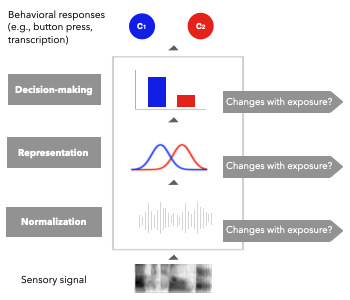
\includegraphics[width=0.6\columnwidth]{../figures/diagrams/overview-of-three-mechanisms2.png}
\caption{Listeners' recognition of speech categories are typically assumed to involve at least three types of mechanisms: 1) the acoustic input is transformed by low-level normalization processes into the perceptual cues that form the input to categorization, 2) linguistic representations describe the mapping between these perceptual and linguistic categories, and 3) decision-making mechanisms allow additional, stimulus-independent, biases to affect recognition. Any of these three mechanisms can in theory be affected by recent experience. While it is now clear \emph{that} recent experience changes the processing of subsequent speech input, most existing findings leave open \emph{which of the three mechanisms underlie these changes.}}\label{fig:overview}
\end{center}
\end{figure}

The majority of recent research on talker-related adaptation has focused on the middle layer, changes in linguistic representations. This includes proposals that attribute exposure effects to ``boundary re-tuning/shifts'' (e.g., \protect\hyperlink{ref-norris2003}{Norris, McQueen, \& Cutler, 2003}; \protect\hyperlink{ref-reinisch2011}{Reinisch, Weber, \& Mitterer, 2011}), ``perceptual/category recalibration'' (e.g., \protect\hyperlink{ref-kraljic-samuel2006}{Kraljic \& Samuel, 2006}; \protect\hyperlink{ref-reinisch-holt2014}{Reinisch \& Holt, 2014}; \protect\hyperlink{ref-samuel2016}{Samuel, 2016}; \protect\hyperlink{ref-vroomen-baart2009}{Vroomen \& Baart, 2009}), ``perceptual retuning'' (\protect\hyperlink{ref-jesse-mcqueen2011}{Jesse \& McQueen, 2011}; \protect\hyperlink{ref-mcqueen2006}{McQueen, Cutler, \& Norris, 2006}; \protect\hyperlink{ref-mitterer2013}{Mitterer, Scharenborg, \& McQueen, 2013}), ``category expansion'' (\protect\hyperlink{ref-schmale2012}{Schmale, Cristia, \& Seidl, 2012}), ``dimension-based statistical learning'' (\protect\hyperlink{ref-idemaru-holt2011}{Idemaru \& Holt, 2011}; \protect\hyperlink{ref-lehet-holt2020}{Lehet \& Holt, 2020}; \protect\hyperlink{ref-liu-holt2015}{Liu \& Holt, 2015}), or ``criteria relaxation'' (\protect\hyperlink{ref-zheng-samuel2020}{Zheng \& Samuel, 2020}). While these proposals are often not further formally specified or modeled (for notable exceptions, see \protect\hyperlink{ref-apfelbaum-mcmurray2015}{Apfelbaum \& McMurray, 2015}; \protect\hyperlink{ref-clayards2008}{Clayards et al., 2008}; \protect\hyperlink{ref-hitczenko-feldman2016}{Hitczenko \& Feldman, 2016}; \protect\hyperlink{ref-kleinschmidt-jaeger2015}{Kleinschmidt \& Jaeger, 2015}; \protect\hyperlink{ref-lancia-winter2013}{Lancia \& Winter, 2013}; \protect\hyperlink{ref-theodore-monto2019}{Theodore \& Monto, 2019}; \protect\hyperlink{ref-xie2021cognition}{Xie et al., 2021}), all of them seem to describe types of changes in representations. For example, ``category shift'' refers to a change in the mean of the cue distribution corresponding to a category, and ``category expansion'' refers to increases in the variance of that distribution. Either of these changes, along with ``cue re-weighting'' or ``learning of new cues,'' can be understood as a consequence of the type of distributional learning that is hypothesized in exemplar (\protect\hyperlink{ref-apfelbaum-mcmurray2015}{Apfelbaum \& McMurray, 2015}; \protect\hyperlink{ref-johnson2006}{Johnson, 2006}), episodic (\protect\hyperlink{ref-goldinger1998}{Goldinger, 1998}), Bayesian inference (\protect\hyperlink{ref-kleinschmidt-jaeger2015}{Kleinschmidt \& Jaeger, 2015}), or neural network models (\protect\hyperlink{ref-lancia-winter2013}{Lancia \& Winter, 2013}). Indeed, recent reviews discuss \emph{what types} of representational changes underlie the effects of recent exposure (e.g., ``category expansion'' vs.~``category shifts''), rather than \emph{whether} representational changes are the actual mechanism underlying the observed results (e.g., \protect\hyperlink{ref-baeseberk2020}{Baese-Berk et al., 2020}; \protect\hyperlink{ref-bent-baeseberk2021}{Bent \& Baese-Berk, 2021}; \protect\hyperlink{ref-schertz-clare2020}{Schertz \& Clare, 2020}). In our own work, we have sometimes made similar assumptions---e.g., when asking whether representational changes can account for adaptation without considering alternative explanations (\protect\hyperlink{ref-kleinschmidt-jaeger2011}{Kleinschmidt \& Jaeger, 2011}, \protect\hyperlink{ref-kleinschmidt-jaeger2012}{2012}, \protect\hyperlink{ref-kleinschmidt-jaeger2016cogsci}{2016}; \protect\hyperlink{ref-kurumada2017}{Kurumada, Brown, \& Tanenhaus, 2017}; \protect\hyperlink{ref-tan2021}{Tan, Xie, \& Jaeger, 2021}).

An absence of contrastive tests, however, means that the same behavioral results could in principle be explained by an alternative mechanism that assumes \emph{no change of linguistic representations}. For instance, if is possible that adaptive changes of responses can be due to low-level, automatic (involuntary) normalization during the early stages of auditory processing (bottom of Figure \ref{fig:overview}) These processes are thought to be pre-linguistic in that they do not refer to categories but rather apply to the acoustic or phonetic cues (\protect\hyperlink{ref-johnson-sjerps2021}{Johnson \& Sjerps, 2021}; \protect\hyperlink{ref-stilp2020}{Stilp, 2020}). In contrast to the assumption that cross-talker variability may be learned and stored, which is fundamental to all the theories of representational changes as described above, theories in normalization assume that listeners remove (or discard) talker variability prior to mapping cues to linguistic categories. \emph{That} such processes help navigate cross-talker variability is widely assumed both in behavioral and neuroimaging research (\protect\hyperlink{ref-irino-patterson2014}{Irino \& Patterson, 2014}; \protect\hyperlink{ref-johnson1990}{Johnson, 1990}; e.g., \protect\hyperlink{ref-kluender1988}{Kluender et al., 1988}; \protect\hyperlink{ref-newman-sawusch1996}{Newman \& Sawusch, 1996}; \protect\hyperlink{ref-pisoni1977}{Pisoni, 1977}; \protect\hyperlink{ref-sawusch-newman2000}{Sawusch \& Newman, 2000}; \protect\hyperlink{ref-sjerps2011}{Sjerps et al., 2011a}; \protect\hyperlink{ref-uddin2020}{Uddin, Reis, Heald, Hedger, \& Nusbaum, 2020}; for discussion, see \protect\hyperlink{ref-barreda2012}{Barreda, 2012}; \protect\hyperlink{ref-magnuson-nusbaum2007}{Magnuson \& Nusbaum, 2007}; \protect\hyperlink{ref-wong2004}{Wong et al., 2004}). However, distinct normalization procedures have mostly been compared to each other (e.g., \protect\hyperlink{ref-adank2004}{Adank, Smits, \& Hout, 2004}; \protect\hyperlink{ref-hoffmanbion-escudero2007}{Hoffmann Bion \& Escudero, 2007}; \protect\hyperlink{ref-kiefte-nearey2019}{Kiefte \& Nearey, 2019}) or against the absence of normalization (\protect\hyperlink{ref-mcmurray-jongman2011}{McMurray \& Jongman, 2011}). They are often not considered as a competing explanation when researchers interpret the results of experiments on accent adaptation, perceptual recalibration, or distributional learning (but see \protect\hyperlink{ref-mullennix-pisoni1990}{Mullennix \& Pisoni, 1990}; \protect\hyperlink{ref-sjerps-reinisch2015}{Sjerps \& Reinisch, 2015}). Only a handful of recent studies have begun to do so for specific contrast types. With some (e.g., English fricatives (\protect\hyperlink{ref-chodroff-wilson2020}{Chodroff \& Wilson, 2020})), low-level auditory normalization has been found to explain human perception of fricatives better than changes in representations.

Yet alternatively, it is possible that \emph{post-linguistic} mechanisms underlie the effects of recent exposure (top of Figure \ref{fig:overview}). Just like normalization is broadly accepted to be part of speech perception, there is little doubt that changes in response biases can affect listeners' interpretation of speech input, or at least the responses they give within experiments. For instance, Clarke-Davidson et al. (\protect\hyperlink{ref-clarkedavidson2008}{2008, p. 605}) define a bias as ``the increased likelihood to give a particular response---such as /s/---given any acoustic input, or the need for less evidence for a particular response'' that ``would help participants make faster word decisions in {[}\ldots{]} ambiguous cases.'' However, such biases are rarely considered in the behavioral literature when analyzing the effects of recent exposure. \emph{When} response biases have been considered (e.g., as {``response equilibration''} in Vroomen and Baart \protect\hyperlink{ref-vroomen-baart2009}{2009}), this explanation tends to be dismissed---prematurely, we believe. One reason for this might be particular result patterns---such as boundary shifts in perceptual recalibration or improved categorization or transcription accuracy in accent adaptation---are considered unlikely to be explained by changes in response biases (or normalization, for that matter).

In investigations into neural systems, in contrast, it is commonplace to isolate prefrontal areas (e.g., \protect\hyperlink{ref-binder2004neural}{Binder, Liebenthal, Possing, Medler, \& Ward, 2004}; \protect\hyperlink{ref-thompson1997role}{Thompson-Schill, D'Esposito, Aguirre, \& Farah, 1997}) as well as the insula and parietal cortex (e.g., \protect\hyperlink{ref-furl2011parietal}{Furl \& Averbeck, 2011}; \protect\hyperlink{ref-keuken2014}{Keuken et al., 2014}) as responsible for perceptual decision-making. Recent studies have begun to investigate whether adaptive changes in speech perception primarily recruit these areas (\protect\hyperlink{ref-erb2013brain}{Erb, Henry, Eisner, \& Obleser, 2013}; \protect\hyperlink{ref-myers-mesite2014}{Myers \& Mesite, 2014}) as opposed to cortical areas associated with phonetic representations (\protect\hyperlink{ref-bonte2017}{Bonte, Correia, Keetels, Vroomen, \& Formisano, 2017}; \protect\hyperlink{ref-luthra2020}{\textbf{luthra2020?}}). For instance, \protect\hyperlink{ref-myers-mesite2014}{Myers \& Mesite} (\protect\hyperlink{ref-myers-mesite2014}{2014}) have suggested that sensitivity to boundary shifts between {[}s{]} and {[}\ipatext{ʃ}{]} emerged in right frontal and middle temporal regions, implicating adjustments of decision-related or attentional criteria downstream from primary auditory cortex. Similarly, a recent work on adaptation to phoneme category substitutions (e.g., {[}s{]} pronounced as {[}\ipatext{ʃ}{]}) found evidence that adaptive processing of such phoneme substitutions engages prefrontal regions, responsible for post-perceptual \emph{repair} mechanisms (\protect\hyperlink{ref-blanco-elorriera2021}{Blanco-Elorrieta, Gwilliams, Marantz, \& Pylkkänen, 2021}): simply put, listeners seemed to initially map the acoustic input onto the wrong category and subsequently corrects the mapping. This was contrasted with the hypothesis that adaptation occurs via returning of the lower level functional connections (e.g., between STG and primary auditory cortex).\footnote{We note that other lines of imaging research have focused on pre-linguistic signal transformations (\protect\hyperlink{ref-sjerps2011listening}{Sjerps, Mitterer, \& McQueen, 2011b}; \protect\hyperlink{ref-zhang2016functionally}{Zhang et al., 2016}) and sensory adaptation (\protect\hyperlink{ref-guediche2015evidence}{Guediche et al., 2015}), including sub-cortical structures (e.g., the brain stem, \protect\hyperlink{ref-skoe2021auditory}{Skoe, Krizman, Spitzer, \& Kraus, 2021}; and cerebellum, \protect\hyperlink{ref-guediche2014}{Guediche, Blumstein, Fiez, \& Holt, 2014}). Compared to the behavioral research we reviewed, it is more common to directly contrast hypotheses that are associated with functionally distinct areas and networks. Like the behavioral research, however, no study to date has examined the three mechanisms in a coherent framework. Studies often adopt stimuli and experimental design that are strongly constrained by particular hypotheses researchers intend to test. The recommendations we provide in General Discussion will help facilitate direct tests across multiple mechanisms.}

Across the behavioral and neuroimaging work, the past research has thus split the underlying process of speech perception (Figure \ref{fig:overview}) in distinct ways. Behavioral studies have begun to distinguish between the (A) normalization and (B) representational changes while continuing to treat (C) post-perceptual decision-making as a factor external to perception. In contrast, the neuroimaging work tends to group (A) and (B) together as happening early in the neural processing stream, functionally distinct from (C) i.e., higher-level, decision-related mechanisms further downstream. To meaningfully link these lines of work, and to better elucidate how human speech perception operates over the variable acoustic input, we need a framework that can encompass (A)-(C) (for a related discussion, see \protect\hyperlink{ref-guediche2014}{Guediche et al., 2014, p. 8}). More specifically, we need a framework to formalize and implement the competing hypotheses about the effects of recent exposure on subsequent speech perception. By testing these predictions using a coherent experimental design, we will be able to test if any of the mechanisms (A)-(C), and \emph{only} that mechanism, can account for adaptive changes seen in human responses.

This motivates the present study. Our long-term goal is to contribute to the development of stronger theories that facilitate decisive comparisons between alternative hypotheses about the mechanisms underlying speech perception (in the tradition of {``strong inference''} approaches to scientific inquiry, \protect\hyperlink{ref-platt1964}{Platt, 1964}). As a first step, we develop a general, unified framework that implements the three distinct theories of adaptive speech perception (i.e., (A)-(C) in Figure \ref{fig:overview}). To anticipate our results, our simulations will demonstrate that the vast majority of existing results do \emph{not} distinguish between three different explanations. We will show this in two highly influential paradigms: so-called \textbf{perceptual recalibration} (e.g., \protect\hyperlink{ref-kraljic-samuel2006}{Kraljic \& Samuel, 2006}; \protect\hyperlink{ref-reinisch-holt2014}{Reinisch \& Holt, 2014}; \protect\hyperlink{ref-samuel2016}{Samuel, 2016}; \protect\hyperlink{ref-vroomen-baart2009}{Vroomen \& Baart, 2009}) and \textbf{(foreign) accent adaptation} (e.g., \protect\hyperlink{ref-bradlow-bent2008}{Bradlow \& Bent, 2008}; \protect\hyperlink{ref-hernandez2019}{Hernández, Ventura-Campos, Costa, Miró-Padilla, \& Ávila, 2019}; \protect\hyperlink{ref-sidaras2009}{Sidaras et al., 2009}; \protect\hyperlink{ref-tzeng2016}{Tzeng, Alexander, Sidaras, \& Nygaard, 2016}; \protect\hyperlink{ref-xie2016jep}{Xie, Theodore, \& Myers, 2016}; \protect\hyperlink{ref-zheng-samuel2020}{Zheng \& Samuel, 2020}). In each, result patterns taken as signature evidence of one mechanism (e.g., changes of representations) could be predicted by \emph{any of the three mechanisms}. To us, and we expect to others in the field, the degree to which this is the case was surprising. These separate lines of research (our own work included) seem to have drawn theoretical conclusions through convention, rather than through strong empirical evidence in favor of a particular mechanism.

As we discussed above, the assumption that our \emph{linguistic representations} adapt to recent exposure has been central to recent breakthroughs in speech perception research (e.g., \protect\hyperlink{ref-hay2019}{Hay, Walker, Sanchez, \& Thompson, 2019}; \protect\hyperlink{ref-kleinschmidt-jaeger2015}{Kleinschmidt \& Jaeger, 2015}; \protect\hyperlink{ref-luthra2020a}{Luthra, Correia, Kleinschmidt, Mesite, \& Myers, 2020}; \protect\hyperlink{ref-sjerps2019}{Sjerps, Fox, Johnson, \& Chang, 2019}). Evidence supporting this assumption has helped shape linguistic theories (\protect\hyperlink{ref-baeseberk2013}{Baese-Berk, Bradlow, \& Wright, 2013}; e.g., \protect\hyperlink{ref-bradlow-bent2008}{Bradlow \& Bent, 2008}; \protect\hyperlink{ref-goldinger-azuma2004}{Goldinger \& Azuma, 2004}; \protect\hyperlink{ref-hay2019}{Hay et al., 2019}; \protect\hyperlink{ref-magnuson-nusbaum2007}{Magnuson \& Nusbaum, 2007}; \protect\hyperlink{ref-tzeng2016}{Tzeng et al., 2016}) as well as theories about the interface between social and linguistic cognition (e.g., \protect\hyperlink{ref-babel2019}{Babel, Senior, \& Bishop, 2019}; \protect\hyperlink{ref-creel-bregman2011}{Creel \& Bregman, 2011}; \protect\hyperlink{ref-foulkes-hay2015}{Foulkes \& Hay, 2015}; \protect\hyperlink{ref-hanulikova2012}{Hanulíková, Alphen, Goch, \& Weber, 2012}; \protect\hyperlink{ref-sumner2014}{Sumner, Kim, King, \& McGowan, 2014}). The empirical indeterminacy that we present calls for a scrutiny of this assumption. Even if one were to take for granted that the three mechanisms in Figure \ref{fig:overview} \emph{jointly} underlie the effects of recent exposure, it remains unclear which of those mechanisms any given results sheds light on. For example, can we conclude from experiments like \protect\hyperlink{ref-clarke-garrett2004}{Clarke \& Garrett} (\protect\hyperlink{ref-clarke-garrett2004}{2004}) that listeners can learn new representations (or at least select some mixture of existing representations) within two minutes of exposure? Or are those results due to normalization, making them substantially less thought-provoking? Also, do the results of perceptual recalibration and accent adaptation stem from the same mechanism(s), or do they reflect different mechanisms (\protect\hyperlink{ref-baeseberk2018}{Baese-Berk, Walker, \& Bradlow, 2018}; \protect\hyperlink{ref-samuel-kraljic2009}{Samuel \& Kraljic, 2009}; \protect\hyperlink{ref-zheng-samuel2020}{Zheng \& Samuel, 2020})? Our comprehensive framework will make it possible to empirically test whether two paradigms that differ substantially in their design, tasks, and ecological validity of the speech stimuli would in fact engage the same mechanism(s).

\begin{figure}[h]
\begin{center}
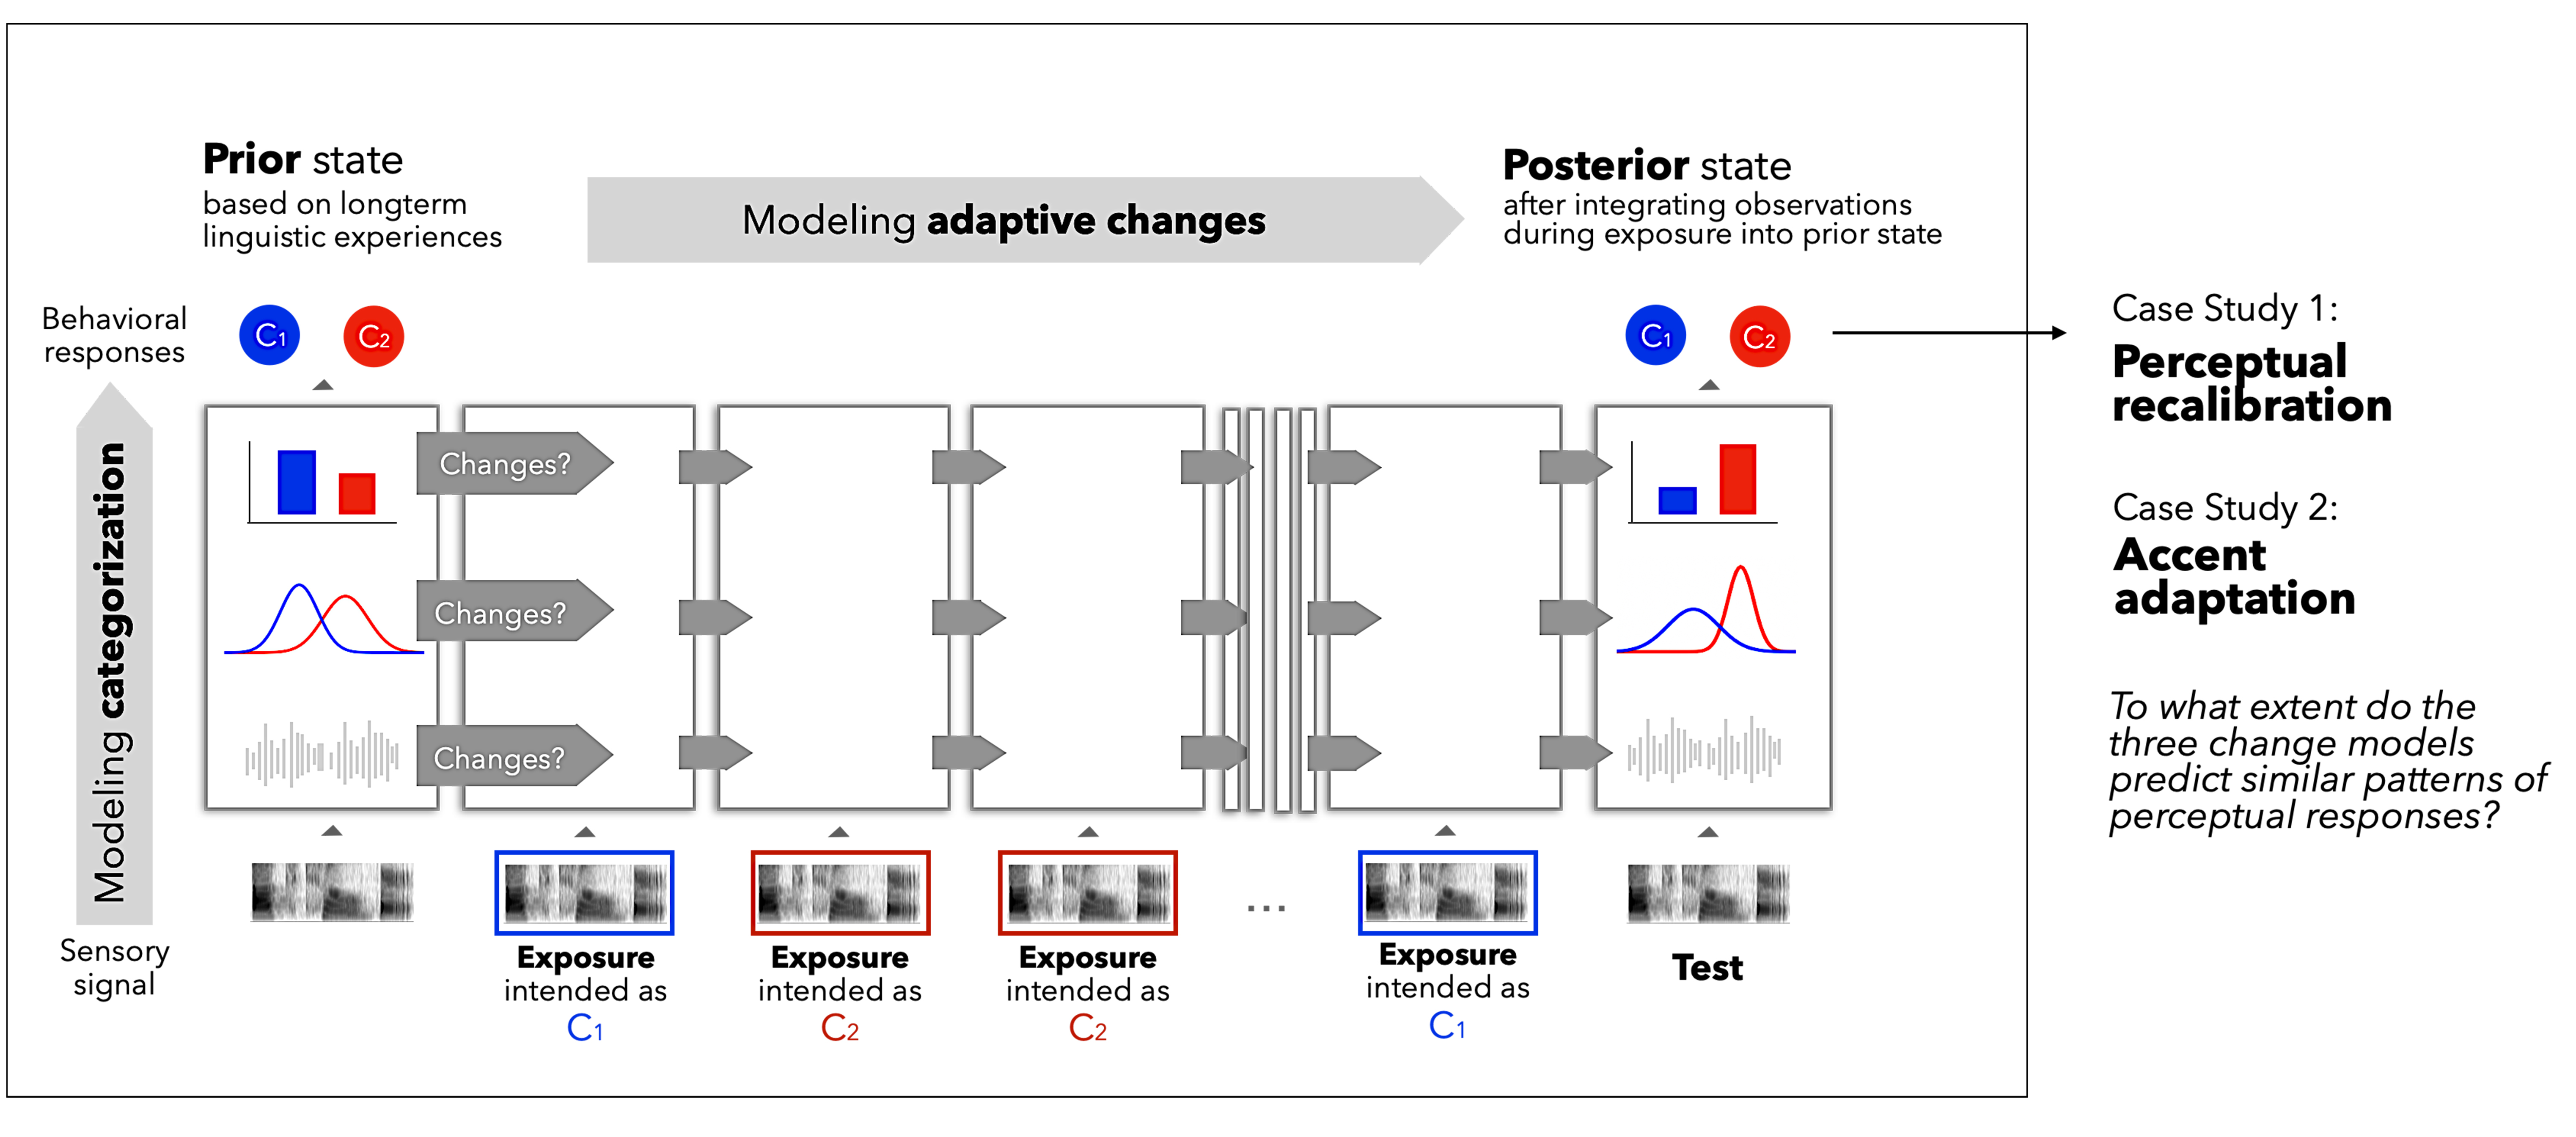
\includegraphics[width=.99\columnwidth]{../figures/diagrams/overview-of-changes.png}
\caption{Overview of our approach. Experiments on the effect of recent exposure on subsequent speech perception tend to involve two phases. An exposure phase manipulates the statistics of speech input between participants. A subsequent test phase assesses the effects of those manipulations on the interpretation of identical speech input. We seek to understand what type of exposure effects each of the three three mechanisms in Figure \ref{fig:overview} can explain. To this end, we specify both a) a {\em categorization model} that describes the interpretation of speech input at any given moment (vertical information flow) and b) {\em change models} for all three mechanism that describe how these parts of the categorization model change as a function of exposure (horizontal information flow). We then use the different change models to compare the predicted consequences of changes to normalization, representations, or response biases.}\label{fig:overview-change}
\end{center}
\end{figure}

The approach we take in this article is illustrated in Figure \ref{fig:overview-change}. We extend the three-pronged process of speech perception (Figure \ref{fig:overview}) to implement \emph{change models} describing how normalization, representations, and responses biases may change with exposure. By training these change models on large-scale production corpora, we simulate adaptive changes of human responses predicted under a given hypothesized mechanism. Our main finding is two fold. First, as we stated above, existing data do not decisively separate their predictions. Present-day conventions in experimental design and analysis severely limit the discriminatory power of behavioral results over the underlying mechanisms. Second, perhaps more significant, it \emph{will} be possible to distinguish the mechanisms from one another if new standards are applied for selection of adaptor/test stimuli as well as for statistical tests. Results of our simulations illuminate when---to what stimuli and under what circumstances---the three mechanisms would provide diverging predictions about adaptive changes of perception. We also learn about how much data will be needed to draw reliable statistical inferences from behavioral data. The general discussion will elaborate on these new standards and how they can be achieved.

All data and code for this article can be downloaded from OSF at \url{https://osf.io/q7gjp/}. This article is written in R markdown, allowing readers to replicate our analyses with the press of a button using freely available software (R, \protect\hyperlink{ref-R}{R Core Team, 2021}; \protect\hyperlink{ref-RStudio}{RStudio Team, 2020}), while changing any of the parameters of our models. Readers can revisit any of the assumptions we make---for example, by substituting alternative models of linguistic representations. The supplementary information (SI, \ref{sec:SI-software}) lists the software/libraries required to compile this document. Beyond our immediate goals here, we hope that this can be helpful to researchers who are interested in developing more informative experimental designs, and to facilitate the interpretation of existing results (see also \protect\hyperlink{ref-tan2021}{Tan et al., 2021}).

\hypertarget{general-discussion}{%
\section{General discussion}\label{general-discussion}}

Listeners' ability to adaptively change their interpretation of the speech signal as a function of recent exposure is now understood to play a central role in spoken language comprehension. Our current case studies suggest that existing results do not distinguish between the three mechanisms. Contrary to common beliefs central to many recent theories of speech perception (\protect\hyperlink{ref-bent-baeseberk2021}{Bent \& Baese-Berk, 2021}; \protect\hyperlink{ref-hay2019}{Hay et al., 2019}; \protect\hyperlink{ref-kleinschmidt-jaeger2015}{Kleinschmidt \& Jaeger, 2015}; \protect\hyperlink{ref-quam-creel2021}{Quam \& Creel, 2021}; \protect\hyperlink{ref-sjerps2019}{Sjerps et al., 2019}), experiments on perceptual recalibration or accent adaptation do \emph{not} offer decisive evidence for a presence or absence of representational changes. This does not, of course, mean that normalization, representation, and decision-making mechanisms always predict similar response patterns---they do not. Nor does it mean that the three mechanisms cannot be distinguished from each other experimentally; It is that current standards of behavioral experiments and data analyses fall short of generating/testing predictions that enable contrastive tests of the mechanisms. In what follows, we discuss insights emerging from the current computational framework and make concrete recommendations for future experiments on speech perception. We then close with discussions on how more decisive empirical tests will facilitate theoretical and empirical advances in uncovering mechanisms of human speech perception.

\hypertarget{methodological-advances-that-can-move-the-field-forward}{%
\subsection{Methodological advances that can move the field forward}\label{methodological-advances-that-can-move-the-field-forward}}

The two case studies highlighted the significant roles of \emph{types} and \emph{strengths} of prior expectations. Given the results we provided, we submit that experimenters ought to operate under the null hypothesis that speech perception is strongly affected by expectations about the distributional realization of linguistic categories based on long-term experiences. This assumption is now shared by most theories of speech perception. It is also emphasized by recent reviews of the field, which highlight and make accessible the role of distributional properties of the speech input (\protect\hyperlink{ref-bent-baeseberk2021}{Bent \& Baese-Berk, 2021}; \protect\hyperlink{ref-kurumada-roettger2021}{Kurumada \& Roettger, 2021}; \protect\hyperlink{ref-quam-creel2021}{Quam \& Creel, 2021}; \protect\hyperlink{ref-schertz-clare2020}{Schertz \& Clare, 2020}). Critically, however, informal reasoning about the consequences of this null hypothesis can quickly gain in complexity, making it more likely that \emph{ad-hoc} or \emph{post-hoc} reasoning results in misleading conclusions. Consider the highly influential study ``The Weckud Wetch of the Wast'' (\protect\hyperlink{ref-maye2008}{Maye et al., 2008}). The study exposed listeners to speech in which the vowel categories had undergone systematic (phonological) shifts. After just 20 minutes of exposure, listeners' interpretation of subsequent speech input from the same talker had changed substantially (for replications and extensions, see also \protect\hyperlink{ref-weatherholtz2014}{Weatherholtz, 2014}). Based on additional control conditions, Maye and colleagues concluded that this finding could not be explained by ``general relaxation of the criterion for what constitutes a good exemplar of the accented vowel category'' but rather argued that participants had learned that the talker's categories were systematically shifted. A recent study revisited this result by formalizing the competing accounts (\protect\hyperlink{ref-hitczenko-feldman2016}{Hitczenko \& Feldman, 2016}). They explicitly encoded assumptions about the listeners' prior expectations (= the ``starting point'' of adaptation) and tested how they can change in response to the input using the same ideal adaptor models that we have employed here (\protect\hyperlink{ref-kleinschmidt-jaeger2015}{Kleinschmidt \& Jaeger, 2015}). They found that the results of Maye et al.~(2008) were just as well, if not better, predicted by a learning model that expanded the categories, rather than shifting them.

Given the computational complexity, an analytical approach like the one we have introduced can be a powerful tool for principled hypothesis testing (see also \protect\hyperlink{ref-apfelbaum-mcmurray2015}{Apfelbaum \& McMurray, 2015}; \protect\hyperlink{ref-sohoglu-davis2016}{Sohoglu \& Davis, 2016}; \protect\hyperlink{ref-tan2021}{Tan et al., 2021}; \protect\hyperlink{ref-theodore-monto2019}{Theodore \& Monto, 2019}; \protect\hyperlink{ref-toscano2018}{Toscano, Toscano, Kleinschmidt, \& Jaeger, 2018}; \protect\hyperlink{ref-xie2021cognition}{Xie et al., 2021}). It provides an alternative to informal reasoning about changes in speech perception. It makes explicit that two types of information affect listeners' interpretation of speech from an unfamiliar talker: (1) the listener's prior expectations based on the statistics of previously experienced speech input; and (2) the statistics of the present speech input relative to those prior expectations. In an exposure-test experiment like those discussed in our case studies, (1) is further divided into two sub-components: (1a) expectations based on the speech statistics experienced prior to the experiment; and (1b) the input experienced during the exposure phase. In other words, the input received during an experiment incrementally changes the prior expectations that the listener brings into a subsequent perceptual response. The three change models we described spell out competing hypotheses about \emph{how} (1b) is integrated with (1a). The categorization model (adapted based on exposure) determines how these changes are expected to affect listeners' responses during the test phase (see Figure \ref{fig:overview-change}). Beyond providing qualitative predictions ({[}CK{]}Here we should probably cite the Pitt paper on parameter space partitioning), the current approach can be used to derive quantitative predictions based on a particular linking hypothesis about mappings between acoustic cues and speech categories.

Below we make four concrete recommendations regarding using the analytical framework to achieve this goal. More specifically, we recommend ways to predict when---to what acoustic-phonetic inputs and after how much exposure---listeners would show adapted responses. By doing this under the three mechanistic hypotheses, we can identify exposure and test items that are expected to yield distinct behavioral responses depending on a mechanism being used (Recommendation 1). Such predictions would have to be formulated and tested along a dimension beyond categorical accuracy (e.g., correct vs.~incorrect identification) or response latency (Recommendation 2). And these predictions need to be spelled out in terms of acoustic-phonetic details of the input (Recommendation 3). Finally, predictive power-simulations using the analytical framework will ensure the statistical power needed for constrastive tests of the three hypothesized mechanisms (Recommendation 4).

\hypertarget{dense-and-targeted-sampling-of-the-stimulus-space}{%
\subsubsection{Dense and targeted sampling of the stimulus space}\label{dense-and-targeted-sampling-of-the-stimulus-space}}

While the change models for all three mechanisms can account for the signature results of perceptual recalibration and accent adaptation paradigms, they do also make different predictions.
Given (1) an estimate of listeners state prior to the experiment and (2) a set of exposure and test stimuli, these predictions are mediated only through the parameters of the change model (e.g., \(\beta_{\pi}\) for changes in response biases), limiting the range of results a change model can account for. That is, instead of merely comparing the ability in which each mechanism captures the \emph{qualitative} pattern of behavioral changes, we can compare the three mechanisms by assessing their accuracy in \emph{quantitatively} predict and explain human responses across a variety of experimental conditions.

Figure \ref{fig:show-model-categorization-3D-plots} illustrates this point for the data from Case Study 2. For each of the three change models, we take the parameters that resulted in the highest accuracy during test, and plot the predicted categorization functions for both exposure conditions. These are the categorization functions that a listener would employ while categorizing test stimuli. Despite the fact that the three change models resulted in qualitatively similar categorization accuracy in Case Study 2, the three models differ in \emph{how} they achieve this accuracy. Specifically, they predict different categorization functions over the VOT-f0 space.



\begin{figure}

{\centering \subfloat[Representations: L1-accented\label{fig:show-model-categorization-3D-plots-1}]{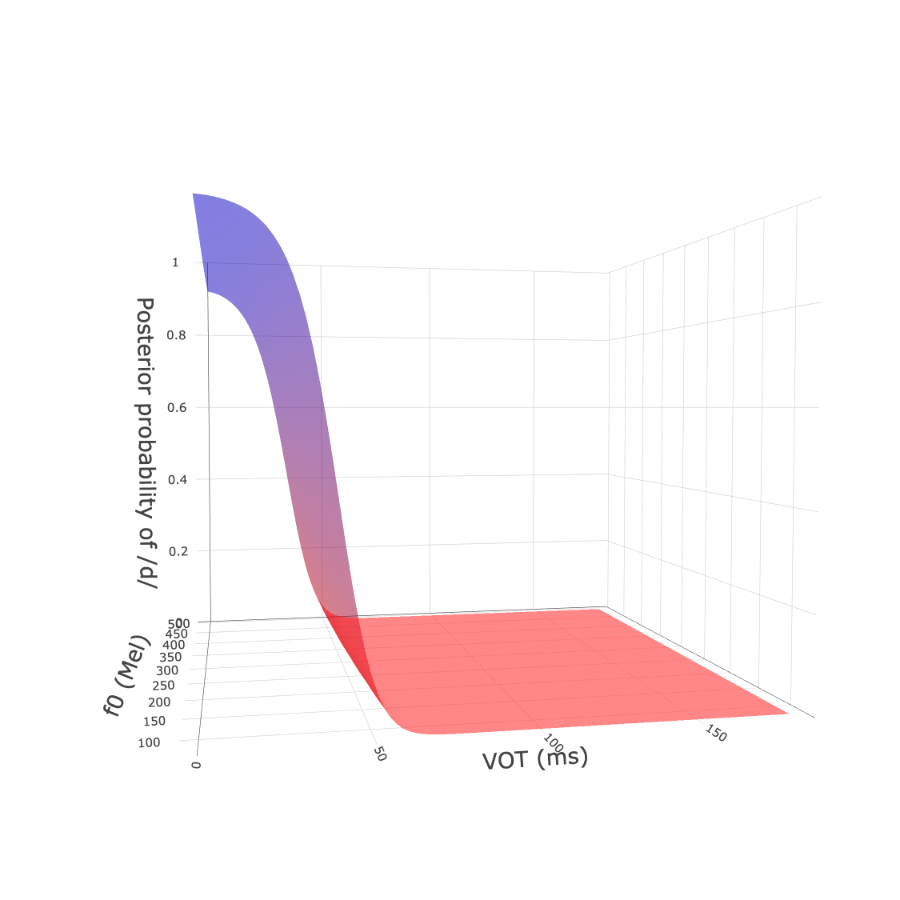
\includegraphics[width=0.33\linewidth,height=0.49\textheight]{../figures/plotly//p.3d.categorization.model_Representations_L1-accented} }\subfloat[Decision making: L1-accented\label{fig:show-model-categorization-3D-plots-2}]{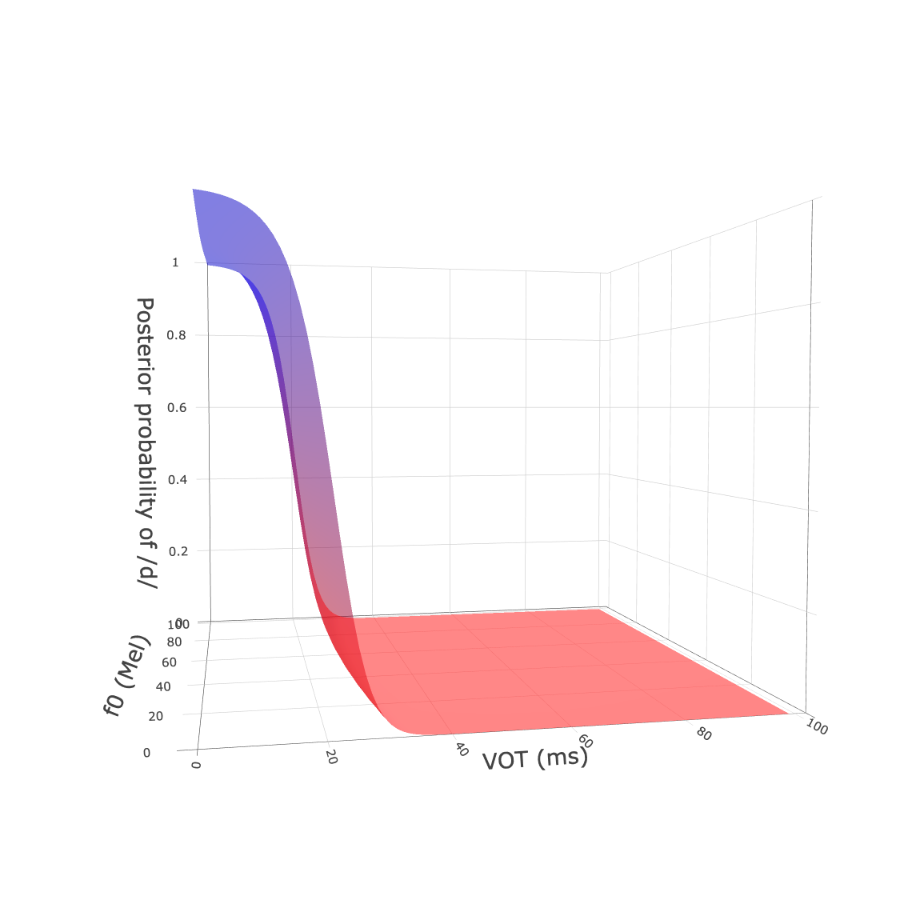
\includegraphics[width=0.33\linewidth,height=0.49\textheight]{../figures/plotly//p.3d.categorization.model_Decision_making_L1-accented} }\subfloat[Normalization: L1-accented\label{fig:show-model-categorization-3D-plots-3}]{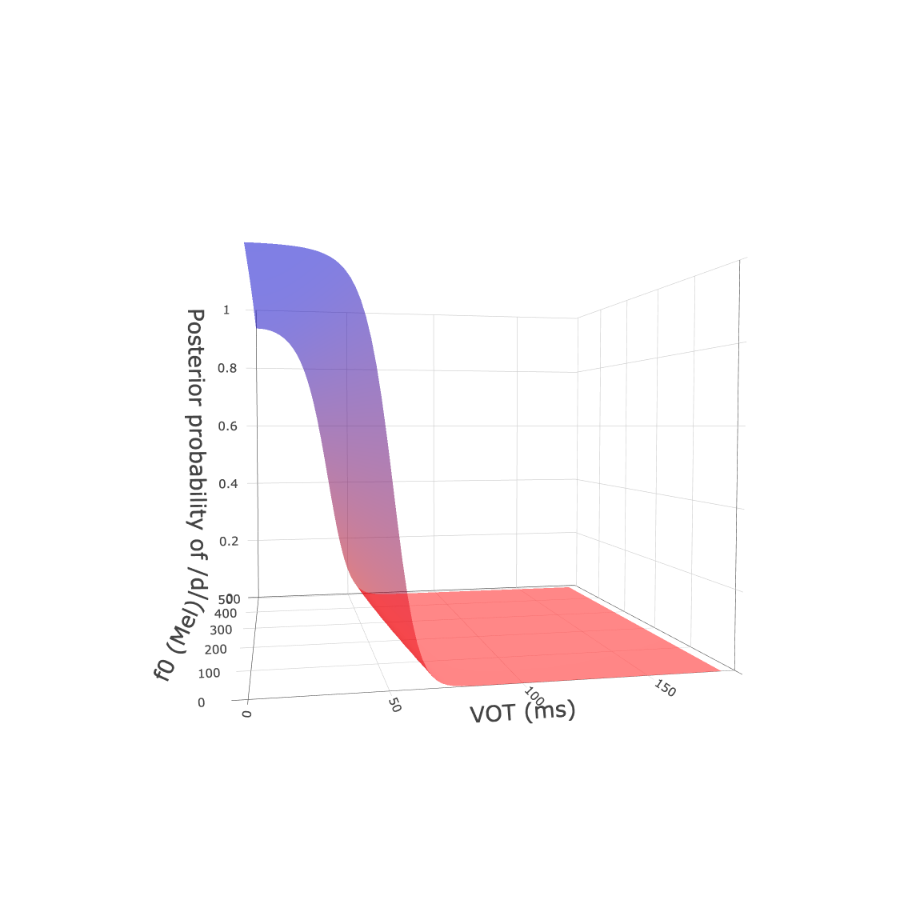
\includegraphics[width=0.33\linewidth,height=0.49\textheight]{../figures/plotly//p.3d.categorization.model_Normalization_L1-accented} }\newline\subfloat[Representations: L2-accented\label{fig:show-model-categorization-3D-plots-4}]{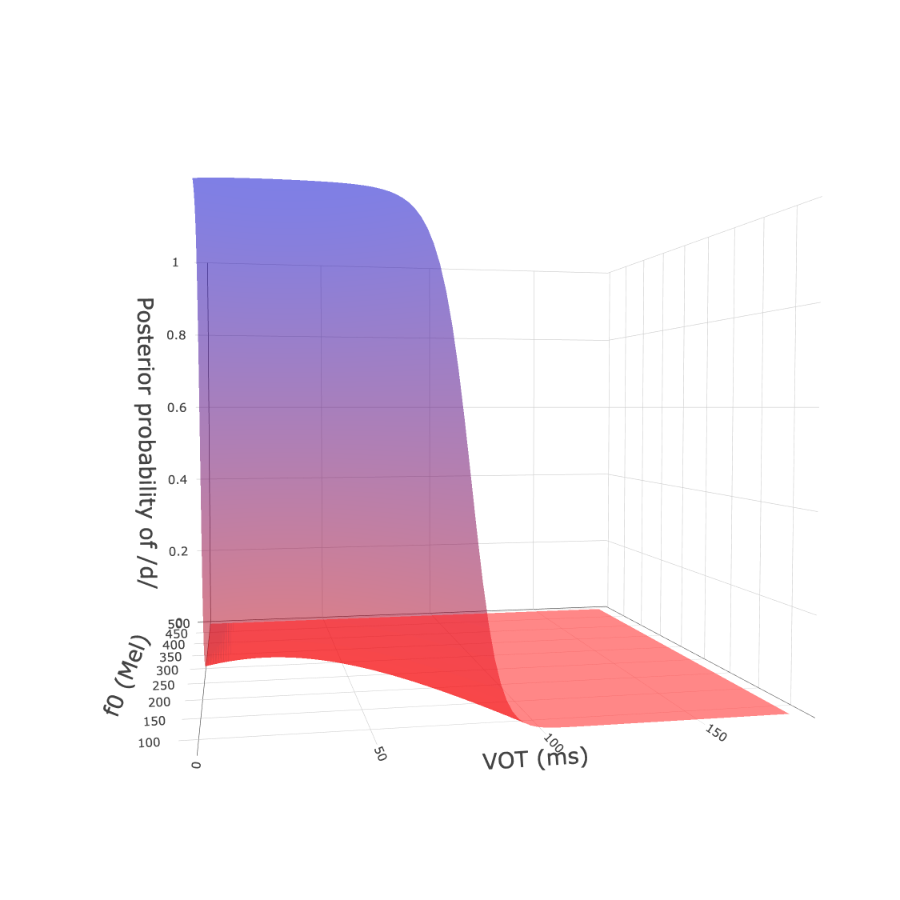
\includegraphics[width=0.33\linewidth,height=0.49\textheight]{../figures/plotly//p.3d.categorization.model_Representations_L2-accented} }\subfloat[Decision making: L2-accented\label{fig:show-model-categorization-3D-plots-5}]{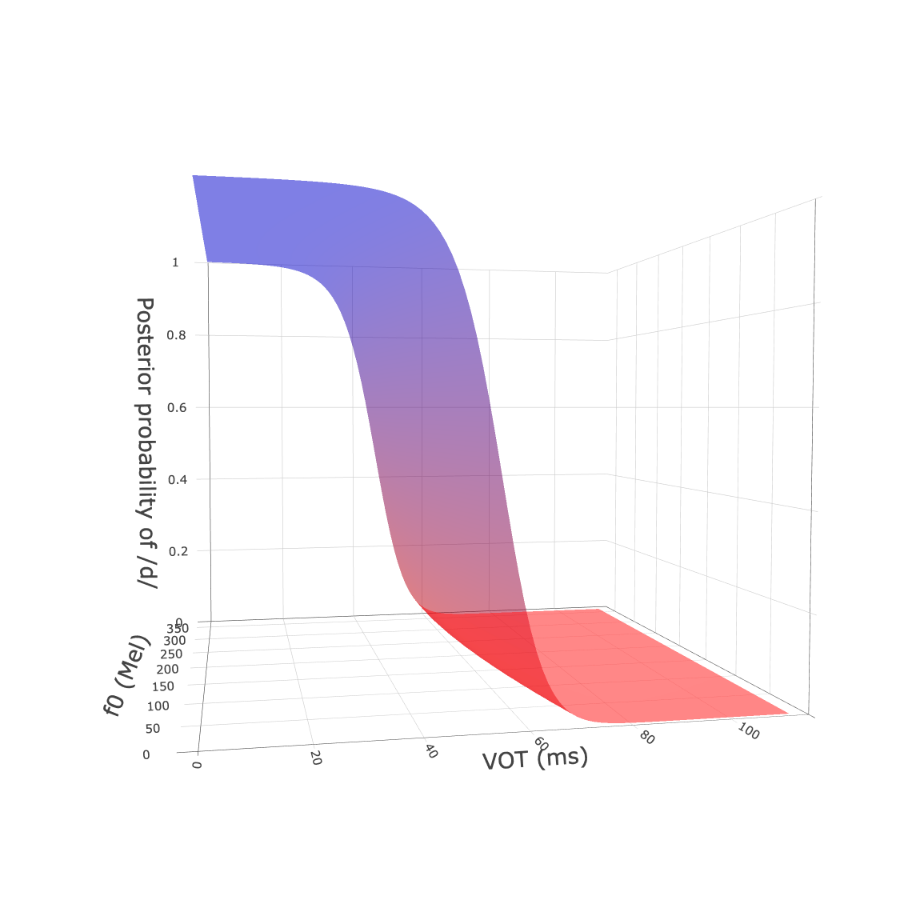
\includegraphics[width=0.33\linewidth,height=0.49\textheight]{../figures/plotly//p.3d.categorization.model_Decision_making_L2-accented} }\subfloat[Normalization: L2-accented\label{fig:show-model-categorization-3D-plots-6}]{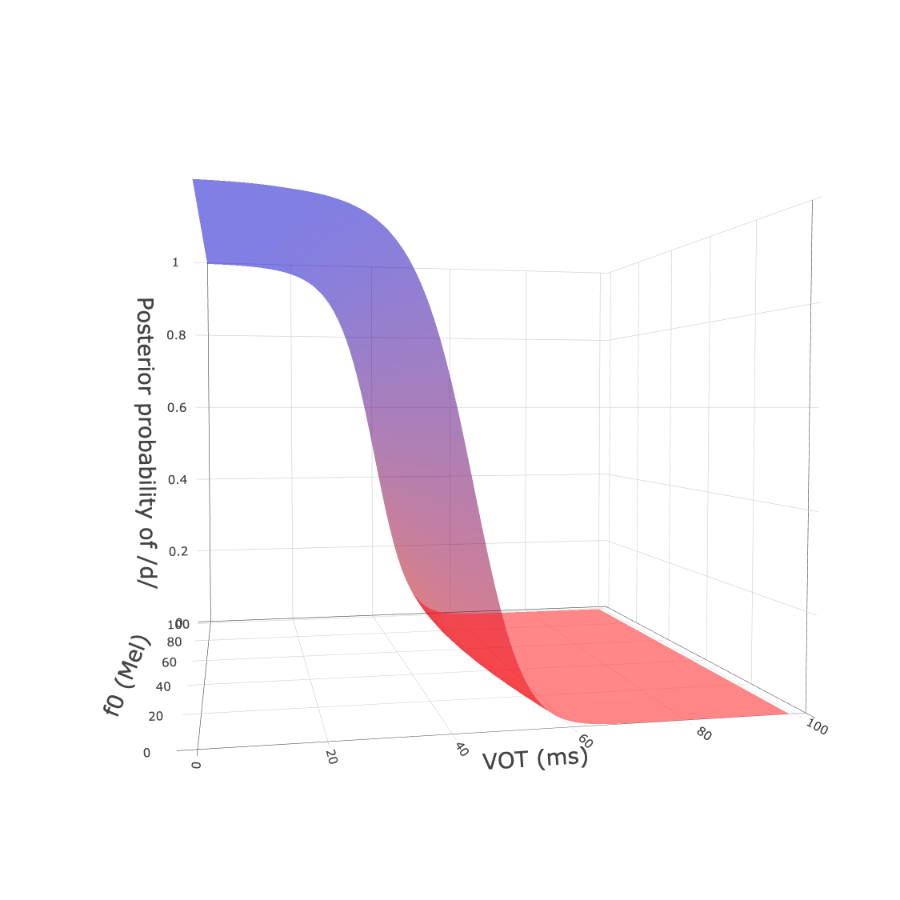
\includegraphics[width=0.33\linewidth,height=0.49\textheight]{../figures/plotly//p.3d.categorization.model_Normalization_L2-accented} }\newline\subfloat[Representations: difference\label{fig:show-model-categorization-3D-plots-7}]{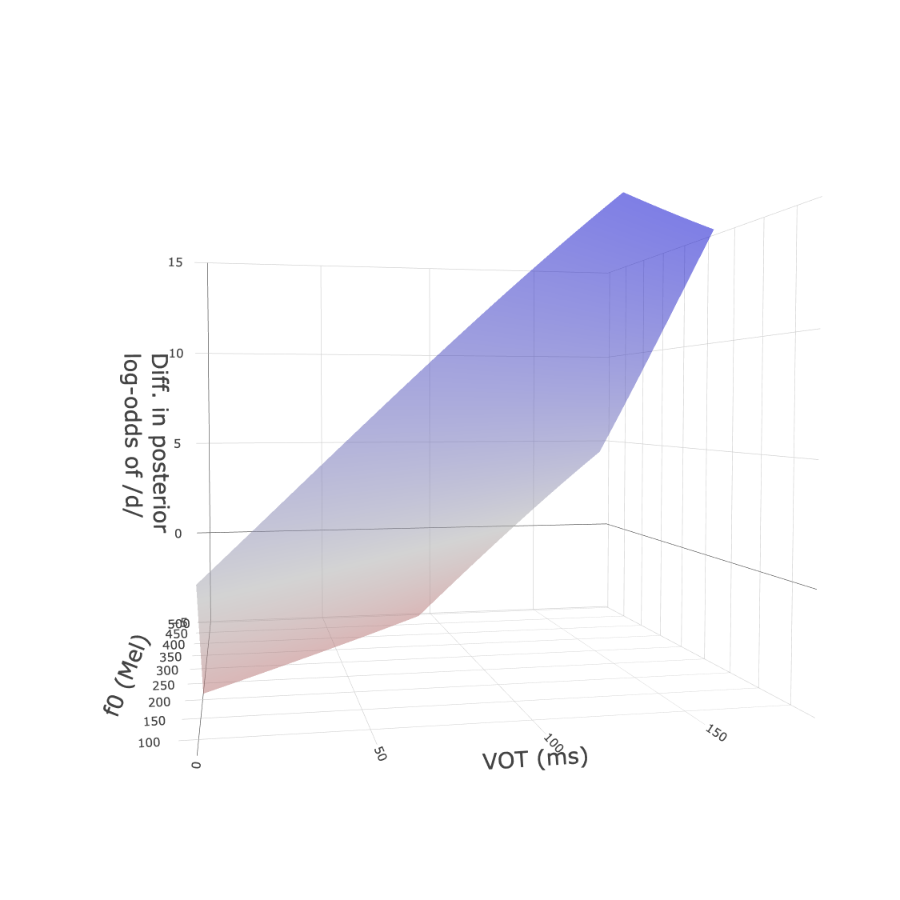
\includegraphics[width=0.33\linewidth,height=0.49\textheight]{../figures/plotly//p.3d.categorization.difference.model_Representations} }\subfloat[Decision making: difference\label{fig:show-model-categorization-3D-plots-8}]{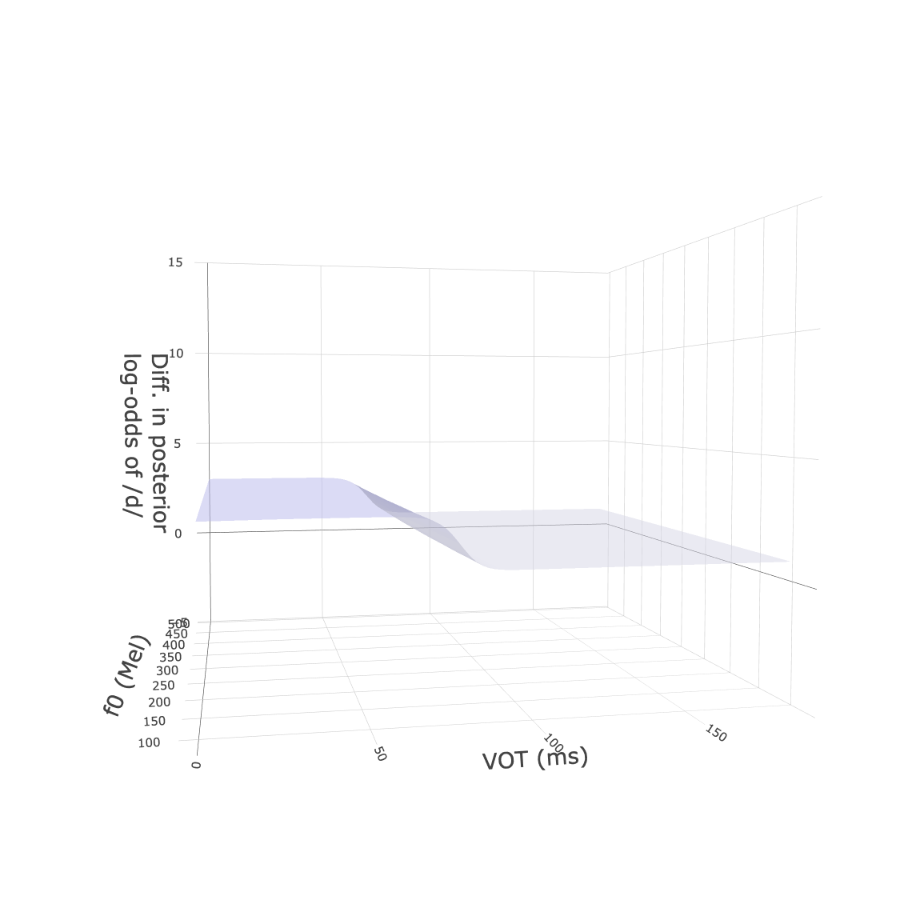
\includegraphics[width=0.33\linewidth,height=0.49\textheight]{../figures/plotly//p.3d.categorization.difference.model_Decision_making} }\subfloat[Normalization: difference\label{fig:show-model-categorization-3D-plots-9}]{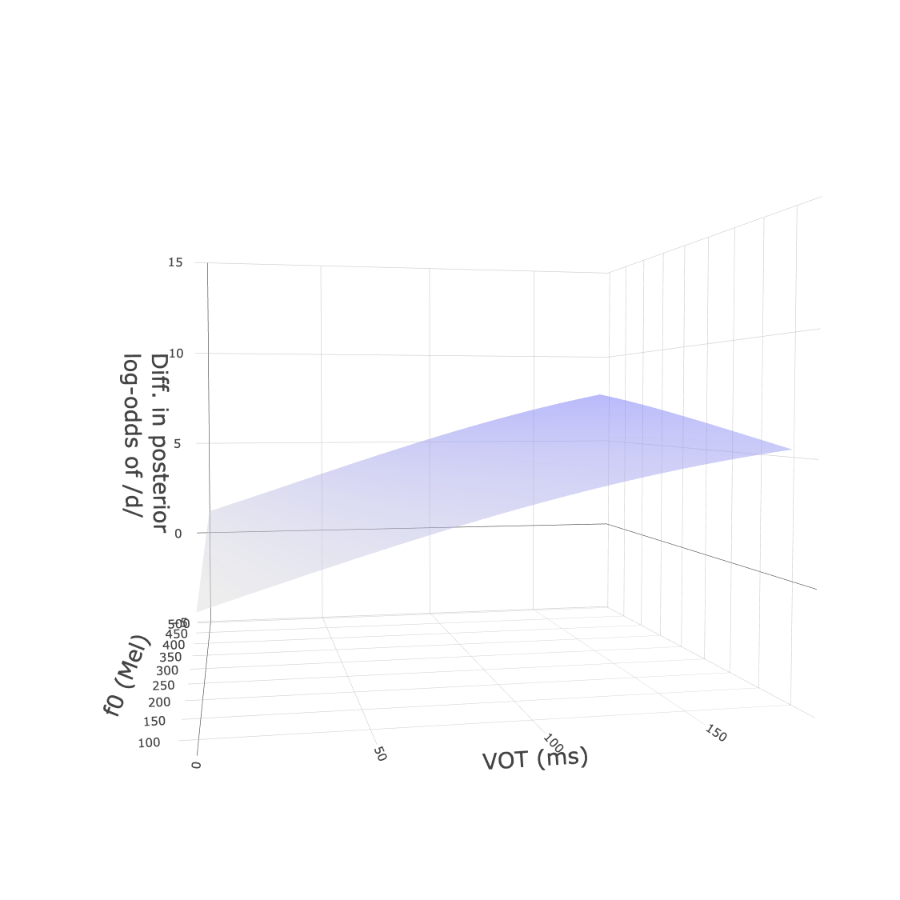
\includegraphics[width=0.33\linewidth,height=0.49\textheight]{../figures/plotly//p.3d.categorization.difference.model_Normalization} }

}

\caption{The three change models predict different categorization functions when applied to the data from Case Study 2. From \textbf{left to right:} predictions for in changes in representations, decision making, and normalization. \textbf{Top:} Predicted categorization functions after L1-accented exposure. \textbf{Middle:} Same but after L2-accented exposure. \textbf{Bottom:} Differences in predicted posterior log-odds of /d/ between the two exposure conditions. Blue indicates higher predicted posterior log-odds of /d/ in the L2-accented exposure condition, relative to the L1-accented exposure condition. Red indicates the opposite. Gray indicates a difference of 0. The three models make distinct predictions about how exposure affects the perception of specific tokens across the VOT-f0 space.}\label{fig:show-model-categorization-3D-plots}
\end{figure}

This points the way to approaches that can more clearly distinguish between the three competing mechanisms. Intuitively, paradigms and analyses should take advantage of the `richness' of the data. Most immediately, this is achieved by moving beyond comparisons that are limited to changes in overall categorization accuracy or processing speed, towards analyses that directly assess the link between the acoustic/phonetic properties of the speech input and listeners' responses. Such approaches are now increasingly common (e.g., \protect\hyperlink{ref-clare2019}{Clare, 2019}; \protect\hyperlink{ref-idemaru-holt2020}{Idemaru \& Holt, 2020}; \protect\hyperlink{ref-kartushina2015}{Kartushina, Hervais-Adelman, Frauenfelder, \& Golestani, 2015}; \protect\hyperlink{ref-kim2020}{Kim, Clayards, \& Kong, 2020}; \protect\hyperlink{ref-liu-holt2015}{Liu \& Holt, 2015}; \protect\hyperlink{ref-schertz2015}{Schertz, Cho, Lotto, \& Warner, 2015}; \protect\hyperlink{ref-wade2007}{Wade et al., 2007}). In order to reliably detect changes in categorization functions, it can be beneficial to more densely sample the acoustic/phonetic space during the test phase. Strategic placement of test stimuli can be used to increase the statistical power to test predicted differences between the different change models (\protect\hyperlink{ref-burchill-jaeger2022}{Burchill \& Jaeger, 2021}). For example, the bottom row of Figure \ref{fig:show-model-categorization-3D-plots} suggests that denser sampling of certain VOT-f0 combinations should make it possible to distinguish between the three change models.

Moving beyond simple contrasts between two exposure conditions can further facilitate comparison between change models. The more exposure conditions an experiment employs, the more accurately and reliably the parameters of the competing change models can be estimated, increasing the power of the model comparison. For instance, \protect\hyperlink{ref-kleinschmidt-jaeger2016cogsci}{Kleinschmidt \& Jaeger} (\protect\hyperlink{ref-kleinschmidt-jaeger2016cogsci}{2016}) and \protect\hyperlink{ref-kleinschmidt2020}{Kleinschmidt} (\protect\hyperlink{ref-kleinschmidt2020}{2020}) created six different between-subject exposure conditions with distinct distributions of VOT. By examining the degree of adaptive changes listeners exhibited in these six conditions, the researchers could estimate their prior expectations more reliably than when only one exposure condition is employed (see also \protect\hyperlink{ref-babel2019}{Babel et al., 2019}; \protect\hyperlink{ref-sumner2011}{Sumner, 2011}). Similarly, incremental testing \emph{within} subjects can increase statistical power to contrast the predictions of different change models. Even when all three change models predict the same \emph{outcome} of adaptation, they can differ in the trajectory of changes they predict. While incremental testing paradigms exist (e.g., \protect\hyperlink{ref-bertelson2003}{Bertelson, Vroomen, \& Gelder, 2003}; \protect\hyperlink{ref-bonte2017}{Bonte et al., 2017}; \protect\hyperlink{ref-vroomen2007}{Vroomen, Linden, Gelder, \& Bertelson, 2007}), they remain under-utilized, and model comparisons based on such experiments remain lacking (but see \protect\hyperlink{ref-kleinschmidt-jaeger2012}{Kleinschmidt \& Jaeger, 2012}).

Either approach---denser sampling of exposure conditions or denser sampling of test tokens---is not limited to paradigms that employ synthesized or otherwise manipulated stimuli (e.g., perceptual recalibration or standard distributional learning paradigms). For example, \protect\hyperlink{ref-chodroff-wilson2020}{Chodroff \& Wilson} (\protect\hyperlink{ref-chodroff-wilson2020}{2020}) took advantage of naturally occurring variability, and created different exposure conditions by selecting different subsets of natural stimuli. This approach strikes a particularly intriguing balance between ecological validity and experimental control.

Finally, comparison across exposure and test conditions might also be achieved through meta-analyses. For example, an ongoing project in our labs pursues this latter approach by constructing a database of over 100,000 categorization responses from dozens of perceptual recalibration experiments on the English /s/-/\ipatext{ʃ}/ contrast. Each of these experiments employs slightly different exposure and test stimuli, potentially increasing the statistical power to distinguish between the competing models. Such item-level meta-analyses benefit immensely from open science standards that facilitate (or even require) the sharing of data in well-documented formats.

\hypertarget{data-analysis-beyond-overall-accuracy-and-speed}{%
\subsubsection{Data analysis beyond overall accuracy and speed}\label{data-analysis-beyond-overall-accuracy-and-speed}}

To take advantage of the richer types of data described in the previous section, it is also necessary to move towards analyses that go beyond changes in the overall accuracy or speed of comprehension. In particular, analyses that directly link relevant acoustic or phonetic properties of the input to listeners' responses strike us as promising. This should take into account that listeners rely on a multitude of cues (e.g., \protect\hyperlink{ref-mcmurray-jongman2011}{McMurray \& Jongman, 2011}) even when the experiment manipulates only one of them. Such analyses could employ the type of model we have described in this study. Alternatively, even simple regression can suffice as long as it employs appropriate linking functions (e.g., logistic regression for categorization, \protect\hyperlink{ref-agresti2019}{Agresti, 2019}; \protect\hyperlink{ref-jaeger2008}{Jaeger, 2008}). This approach is now increasingly common, taking advantage of stimulus-level variability within and across conditions to test hypotheses. These regression analyses can be expanded to accommodate lapse rates and response biases (e.g., \protect\hyperlink{ref-clayards2008}{Clayards et al., 2008}; \protect\hyperlink{ref-kleinschmidt2020}{Kleinschmidt, 2020}), and can be fit in standard statistics software (e.g., through \texttt{brms} \protect\hyperlink{ref-burkner2017}{Bürkner, 2017} or other libraries in \texttt{R}). A comprehensive introduction to such models is provided in \protect\hyperlink{ref-wichmann-hill2001}{Wichmann \& Hill} (\protect\hyperlink{ref-wichmann-hill2001}{2001}).

Indeed, there are direct connections between the model we have employed here and lapsing logistic regression. For example, two Gaussian categories along a phonetic continuum result in linear effect of the continuum on the posterior log-odds of the categories if the two categories have identical variance, but linear + quadratic if the two categories have unequal variance (e.g., \protect\hyperlink{ref-kleinschmidt-jaeger2015}{Kleinschmidt \& Jaeger, 2015}; \protect\hyperlink{ref-kronrod2016}{Kronrod, Coppess, \& Feldman, 2016}). This prediction can only be appreciated if logistic regression is employed for the analysis of 2AFC categorization tasks, rather than ANOVA or similar methods. \protect\hyperlink{ref-schertz-clare2020}{Schertz \& Clare} (\protect\hyperlink{ref-schertz-clare2020}{2020}) provides an excellent overview of how standard regression analyses can be---and have been---used to assess the effects multiple phonetic cues on listeners' responses.

\hypertarget{advance-standards-of-data-annotation-reporting-and-sharing}{%
\subsubsection{Advance standards of data annotation, reporting, and sharing}\label{advance-standards-of-data-annotation-reporting-and-sharing}}

Theories of speech perception now agree that the distribution of acoustic or phonetic cues in the input is critical to understanding speech perception. As described above, a deeper understanding of how recent exposure comes to shape speech perception requires that researchers acknowledge this link, and advance their standards of data reporting accordingly. We recommend that it should become standard for studies on speech perception to report the relevant phonetic properties of their stimuli. For the paradigms like the ones we have discussed here, this would include phonetic annotations of both the exposure and test stimuli. As an added benefit, phonetic annotations also allow more sophisticated and natural stimulus manipulation (see the insightful critique offered in \protect\hyperlink{ref-theodore2021}{Theodore, 2021}).

In our view, such annotations entail a manageable effort: perception experiments typically employ a small number of speech stimuli that are repeated for each participant. A typical perceptual recalibration experiment would require the annotation of less than 100 isolated word recordings. A large study on accent adaptation like Bradlow and Bent's (2008) Experiment 2 would require the annotation of about 1000 sentences. Studies on phonetic production regularly annotate data sets many times larger. These efforts towards a more open, collaborative science can further be supported by clear standards for reproducibility and software developments that aid phonetic annotation and data sharing (e.g., \protect\hyperlink{ref-cassidy-schmidt2017}{Cassidy \& Schmidt, 2017}; \protect\hyperlink{ref-picoral2021}{Picoral, Staples, \& Reppen, 2021}; \protect\hyperlink{ref-roettger2019}{Roettger, Winter, \& Baayen, 2019}; \protect\hyperlink{ref-winkelmann2017}{Winkelmann, Harrington, \& Jänsch, 2017}). If annotations are not reported and shared---and ideally even if they are---then all audio recordings should be shared in an open and accessible way (e.g., OSF). This will require perception researchers to elicit recordings in ways that gives them the consent to distribute these recordings for the purpose of scientific inquiry. In other words, perception researchers would have to follow the same standards that researchers working on language production are expected to follow.

\hypertarget{simulation-and-power-analysis-prior-to-conducting-testing}{%
\subsubsection{Simulation and power analysis prior to conducting testing}\label{simulation-and-power-analysis-prior-to-conducting-testing}}

As made clear in the case studies, it is critical to formulate clear linking hypotheses that describe the mapping from the acoustic/phonetic input to perception (see also \protect\hyperlink{ref-apfelbaum-mcmurray2015}{Apfelbaum \& McMurray, 2015}; \protect\hyperlink{ref-tanenhaus2004}{Tanenhaus, 2004}). Analytical frameworks like the one we introduced here can be used to estimate expected sizes of effects before conducting an experiment. Unlike commonly used power estimates---which assume expected effect sizes (based on previous work or arbitrarily set to e.g., ``moderate'')---a fully specified change model can derive predicted effect sizes under a hypothesized mechanism. This will make power-analyses less arbitrary and more informative.

In addition to phonetically annotated exposure and test stimuli, such power analyses require estimates of listeners' prior expectations at the start of the experiment. Because these estimates aim to capture expectations based on input previously experienced throughout listeners' lives, these estimates entail substantially more effort than the annotation of experimental stimuli. Fortunately, large and phonetically annotated databases of the speech variety assumed to have been the primary input of the listeners under study. Such databases are now available for an increasing number of phonological contrasts and languages (e.g., \protect\hyperlink{ref-chodroff-wilson2018}{Chodroff \& Wilson, 2018}; \protect\hyperlink{ref-clopper-pisoni2006}{Clopper \& Pisoni, 2006}; \protect\hyperlink{ref-hillenbrand1995}{Hillenbrand, Getty, Clark, \& Wheeler, 1995}; \protect\hyperlink{ref-newman2001}{Newman et al., 2001}; \protect\hyperlink{ref-theodore2009}{Theodore, Miller, \& DeSteno, 2009}; \protect\hyperlink{ref-xie-jaeger2020}{Xie \& Jaeger, 2020}, among many others). One caveat is that many of these databases either are representative only of a subset of the varieties that an average speaker of a language has plausibly been exposed to, or contain very little data for each variety. In particular, databases that contain both a large number of talkers, and a large number of tokens per talker, continue to be the exception. Researchers need to carefully consider these implications when employing databases. In some cases, researchers might find that the best way forward is to collect phonetically annotated data that meets the specific requirements for their study. \protect\hyperlink{ref-xie2021cognition}{Xie et al.} (\protect\hyperlink{ref-xie2021cognition}{2021}), for instance, collected \textasciitilde3000 production tokens of prosodic categories and used them to model listeners' responses in a perception experiment. We have also found that sometimes phonetically annotated data from a single typical talker can be sufficient to get started---e.g., to gain an initial understanding of one's results (\protect\hyperlink{ref-tan2021}{Tan et al., 2021}) or to conduct power simulations.

One alternative option is to eschew phonetically annotated data in favor of computational methods that work with the raw signal or some automatically obtained transformation of the raw data (such as Mel-Frequency Cepstral Coefficents, (MFCC) \protect\hyperlink{ref-Mermelstein1976}{Mermelstein, 1976}). Such models have been developed for automatic speech recognition (for an earlier review, see \protect\hyperlink{ref-jurafsky-martin2000}{Jurafsky \& Martin, 2000}) and have been employed to model human language acquisition (\protect\hyperlink{ref-dupoux2018}{Dupoux, 2018}; \protect\hyperlink{ref-feldman2013}{Feldman, Myers, White, Griffiths, \& Morgan, 2013}; \protect\hyperlink{ref-toscano-mcmurray2010}{Toscano \& McMurray, 2010}; \protect\hyperlink{ref-vallabha2007}{Vallabha, McClelland, Pons, Werker, \& Amano, 2007}). More recently, they have also been applied to address questions about the effects of recent exposure (\protect\hyperlink{ref-richter2017}{Richter, Feldman, Salgado, \& Jansen, 2017}). The general framework we have described here can be combined with such models.

\hypertarget{distinguishing-between-the-mechanisms-how-will-that-advance-theories-of-speech-perception}{%
\subsection{Distinguishing between the mechanisms -- How will that advance theories of speech perception?}\label{distinguishing-between-the-mechanisms-how-will-that-advance-theories-of-speech-perception}}

Being able to distinguish between the mechanisms of adaptation has potentially far-reaching implications. Besides the two classes of experimental paradigms we detailed above, there are a wider range of behavioral and neuro-imaging results cited as evidence for or against a particular mechanism underlying accurate and robust speech perception. Most of these studies are, however, vulnerable to the empirical indeterminacy. Each study tests one hypothesis at a time, leaving it open whether the same results could be explained by an alternative mechanism. Implementing contrastive tests can thus help synthesize diverse lines of work, consolidating efforts for theoretical and empirical advances in the field.

\hypertarget{behavioral-study-results}{%
\subsubsection{Behavioral study results}\label{behavioral-study-results}}

Theories that assume changes of representations find support in episodic memories stored and retrieved in relation to a particular context. These memories include the (inferred) physiology (\protect\hyperlink{ref-krauss2002}{Krauss, Freyberg, \& Morsella, 2002}) or social identity of a talker can affect how her speech is processed and interpreted (e.g., regional origin, \protect\hyperlink{ref-hay-drager2010}{Hay \& Drager, 2010}; \protect\hyperlink{ref-niedzielski1999}{Niedzielski, 1999}; sex, \protect\hyperlink{ref-johnson1999}{Johnson, Strand, \& D'Imperio, 1999}; \protect\hyperlink{ref-strand1999}{Strand, 1999}; age, \protect\hyperlink{ref-walker-hay2011}{Walker \& Hay, 2011}; \protect\hyperlink{ref-skoogwaller2015}{Waller, Eriksson, \& Sörqvist, 2015}; and individual identity, \protect\hyperlink{ref-nygaard1994}{Nygaard et al., 1994}; \protect\hyperlink{ref-remez2018}{Remez et al., 2018}). These and other effects of the situational context (e.g., being in a car, \protect\hyperlink{ref-hay2017}{Hay, Podlubny, Drager, \& McAuliffe, 2017}) have been taken to suggest that listeners have implicit representations that encode expectations about talkers and types of talkers. These findings do, however, leave open whether these expectations relate to pre-linguistic normalization or to linguistic categories (see also discussion of {``relativization''} in \protect\hyperlink{ref-apfelbaum-mcmurray2015}{Apfelbaum \& McMurray, 2015, pp. 936--938}). They also leave open to what extent recent (e.g., within-experiment) experience affects speech perception through the same mechanisms that underlie the effects of inferred physiology or social identity. (This includes the question of whether and how recent experiences can lead to the learning of new linguistic representations. (e.g., Can listeners \emph{learn} characteristics of a talker within 2 mins of exposure?) The approach and the recommendations provided above will make it possible to explicitly test these subtly distinct possibilities, which have not thus far possible.

Similarly, there are other types of results that seem to be difficult to explain through C-CuRE normalization or changes in responses biases. Perhaps one of the most important studies in this regard is \protect\hyperlink{ref-clayards2008}{Clayards et al.} (\protect\hyperlink{ref-clayards2008}{2008}) and subsequent replications and extensions (\protect\hyperlink{ref-bejjanki2011}{Bejjanki, Clayards, Knill, \& Aslin, 2011}; \protect\hyperlink{ref-nixon2016}{Nixon, Rij, Mok, Baayen, \& Chen, 2016}; \protect\hyperlink{ref-theodore-monto2019}{Theodore \& Monto, 2019}). Clayards and colleagues found that categorization responses can be affected by changes of the category variances, without changes in the category means. Specifically, participants that were exposed to /b/ and /p/ categories with larger variance along VOT exhibited more shallow categorization slopes than participants who were exposed to /b/ and /p/ categories with smaller variance (but the same means as the other condition).

This result is predicted by distributional learning accounts of representational changes (as discussed by \protect\hyperlink{ref-clayards2008}{Clayards et al., 2008}; \protect\hyperlink{ref-kleinschmidt-jaeger2015}{Kleinschmidt \& Jaeger, 2015}) but is not as easily explained by C-CuRE normalization. It does not, however, rule out explanations in terms of other normalization. For example, normalization that standardizes cues relative to expectations, in addition to centering them---which we might call \emph{S}-CuRE (for ``standardizing'')---should be able to account for the findings of Clayards et al.~(2008). Such standardization is part of several of the most influential approaches to formant normalization that have been proposed for the perception of vowels (\protect\hyperlink{ref-johnson2020}{Johnson, 2020}; \protect\hyperlink{ref-lobanov1971}{Lobanov, 1971}; \protect\hyperlink{ref-monahan-idsardi2010}{Monahan \& Idsardi, 2010}). The findings of Clayards et al.~(2008) might also be accounted for by changes in response biases provided that the lapse rate is not zero: recall that changes in responses biases can have non-additive effects when the lapse rate is non-zero (Section \ref{sec:change-bias}). And non-zero lapse rates were indeed observed by Clayards et al.~(2008, Figure 3B and footnote 2). Changes in response biases could thus potentially account for changes in the slope of categorization functions---the result observed in Clayards et al.~(2008).

Conversely, there are clasesse of results that have been traditionally linked to the normalization mechanism. Many of these have utilized non-linguistic stimuli as adaptors (\protect\hyperlink{ref-holt2005}{Holt, 2005}, \protect\hyperlink{ref-holt2006}{2006}; \protect\hyperlink{ref-huang-holt2011}{Huang \& Holt, 2011}). An observation that exposure to non-linguistic sounds (e.g., pure tones) changes subsequent recognition seems to be hard to explain through changes in linguistic representations. Traditionally, such a result is often used to argue for the involvement of a general, pre-lingusitic auditory mechanism. These findings have, however, been challenged (\protect\hyperlink{ref-pitt2016}{Pitt, Szostak, \& Dilley, 2016}). The current approach can be used to explicitly model the effects of accumulating exposure to non-linguistic inputs in terms of representational changes or decision-making, for a direct comparison of their fit to human response behaviors. Furthermore, the modeling approach can be straightforwardly extended to test whetgher a \emph{combination} of mechanisms could approximate human data. This will help address the intuitive, yet computationally-complex, possibility that human listeners may store and learn distributional characteristics of speech categories in an acoustic-phonetic space \emph{post} normalization (\protect\hyperlink{ref-xie2021cognition}{Xie et al., 2021}).

\hypertarget{neuro-imaging-study-results}{%
\subsubsection{Neuro-imaging study results}\label{neuro-imaging-study-results}}

The primary goal of the current investigation has been to make strong inference through behavioral testing. Once achieved, it will facilitate more targeted neuro-imaging research. As discussed in the introduction, shifted categorization boundaries in response to the same physical input have been associated with multiple regions, such as early auditory regions (anterior PT, \protect\hyperlink{ref-kilianhutten2011}{Kilian-Hütten, Vroomen, \& Formisano, 2011}), regions implicated in phoneme classification (posterior STG/STS, \protect\hyperlink{ref-bonte2017}{Bonte et al., 2017}; \protect\hyperlink{ref-myers-mesite2014}{Myers \& Mesite, 2014}; \protect\hyperlink{ref-ullas2020}{Ullas, 2020}), as well as regions for talker identity processing (right temporal regions, \protect\hyperlink{ref-luthra2020a}{Luthra et al., 2020}). The left parietal lobe and the insula, which are implicated in perceptual decision-making (e.g., \protect\hyperlink{ref-dacremont2013}{d'Acremont, Schultz, \& Bossaerts, 2013}; \protect\hyperlink{ref-keuken2014}{Keuken et al., 2014}), have also been shown to exhibit distinct activation for different exposure conditions (\protect\hyperlink{ref-bonte2017}{Bonte et al., 2017}; \protect\hyperlink{ref-myers-mesite2014}{Myers \& Mesite, 2014}; \protect\hyperlink{ref-ullas2020}{Ullas, 2020}). As in behavioral experiments, existing results leave open which neural networks are responsible for the behavioral changes observed after recent exposure. Even a significant activation of a given brain region can be associated with functionally-distinct sources. For instance, the activation of left parietal lobe might reflect its general role in perceptual decision making (e.g., \protect\hyperlink{ref-dacremont2013}{d'Acremont et al., 2013}; \protect\hyperlink{ref-keuken2014}{Keuken et al., 2014}), or it could be due to a more specific role in phonological processing (e.g., processing abstract category information, \protect\hyperlink{ref-guediche2014}{Guediche et al., 2014}).

One limitation of these works is that the conclusion is based primarily on a binary distinction in a brain region's activation pattern (e.g., activity between categorization trials that a /d/ response is made and those in which a /t/ response is made for the same stimulus). More recently, neuroimaging studies have started to approach questions about the underlying neural mechanisms through multivariate analyses. These analyses are crucial for identifying the encoding of perceptual experiences across a distinct array of experimental conditions. Multivariate analyses can also be more sensitive in detecting fine-grained patterns \emph{within} regions responsible for multiple cognitive demands (e.g., \protect\hyperlink{ref-bonte2017}{Bonte et al., 2017}; \protect\hyperlink{ref-luthra2020a}{Luthra et al., 2020}). The methodological recommendations we made above may help generate behavioral responses that enable multivariate analyses required for further dissociation among regions functionally responsible for exposure-driven changes.

Furthermore, better linking stimulus features and response changes can help synthesize insights from behavioral and neuro-imaging studies and help generate new predictions. For instance, a recent study by \protect\hyperlink{ref-zheng-samuel2020}{Zheng \& Samuel} (\protect\hyperlink{ref-zheng-samuel2020}{2020}) used the two behavioral paradigms we adopted above: perceptual recalibration to L1-accented speech (as in Case Study 1) and adaptation to L2-accented speech (as in Case Study 2). They did so to test if there is any within-subject correlation in subjects' task performances. If there is, that would suggest that there is a common mechanism underlying both types of adaptive changes in perceptual responses. For the accent adaptation task, they used authentic Mandarin-accented speech, wherein {[}\ipatext{θ}{]} (as in \emph{thick}) was pronounced as {[}s{]} (as in \emph{sick}). Zheng and Samuel (2020) reported that: (a) listeners indeed improved their recognition of these substituted phonemes with accumulating exposure to a Mandarin-accented talker; while (b) there was no within-subject link between performances in the two tasks. Subjects who were more likely to adapt to the phoneme substitution were not necessarily more likely to show a categorization boundary shift. In fact, this corresponds to a recent neuro-imaging results by \protect\hyperlink{ref-blanco-elorriera2021}{Blanco-Elorrieta et al.} (\protect\hyperlink{ref-blanco-elorriera2021}{2021}). They argued that recognition of a substituted phoneme (e.g., {[}s{]} pronounced as {[}\ipatext{ʃ}{]}) relies on post-perceptual decision-making, rather than calibration at an upstream in auditory processing. Perhaps, adaptation to a non-native accent may not involve stimulus-dependent changes at all.

Alternatively, the different mechanisms might trade-off depending on a relative (expected) recognition benefit achieved through each. A full-scale substitution between the expected and observed category realizations (e.g., {[}\ipatext{θ}{]} as {[}s{]} in \protect\hyperlink{ref-zheng-samuel2020}{Zheng \& Samuel} (\protect\hyperlink{ref-zheng-samuel2020}{2020}) and {[}s{]} as {[}\ipatext{ʃ}{]} in \protect\hyperlink{ref-blanco-elorriera2021}{Blanco-Elorrieta et al.} (\protect\hyperlink{ref-blanco-elorriera2021}{2021})) reduces the effectiveness of normalization because the two categories are acoustically indistinguishable. It also makes changes of represenations relatively costly and proportionally less effective: means and variances of the categories overlap with one another and learning them does not necessarily improve the chance of correct recognition. In this scenario, at least in initial moments of exposure, changing decision biases alone would lead to improved recognition of categories intended by the talker. Put differently, listeners may not be using different mechanisms for different tasks (e.g., perceptual recalibration vs.~accent adaptation, or accommodating L1- vs.~L2-accented speech). Rather, they may be adopting \emph{a mechanism that would efficiently lead to recognition improvements given the stimulus features and their distributions over speech categories}. Testing this hypothesis would require careful parameterization of acoustic-phonetic features, categories/contrasts, and tasks within subjects. The current analytical framework, and the new standards of experimental design and analyses laid out above, will be indispensable for this endevour.

Finally, Another promising avenue is to pair temporally-sensitive techniques with imaging methods with good spatial resolution. For instance, studies using a combination of EEG and MEG have identified key regions that regulate perceptual learning of degraded speech by responding to manipulations of either low-level signal clarity or high-level prior knowledge of the speech content (\protect\hyperlink{ref-sohoglu-davis2016}{Sohoglu \& Davis, 2016}; \protect\hyperlink{ref-sohoglu-davis2020}{Sohoglu \& Davis, 2020}).

\hypertarget{conclusion}{%
\section{Conclusion}\label{conclusion}}

While there is now a convergence of different approaches---including both behavioral and neuroimaging paradigms---existing findings leave open what neural and cognitive mechanisms underlie adaptive changes in speech perception. In this context, our case studies support two take-home points: i) that far less is known about what mechanisms yield the results of our experiments than seems to be often assumed; and ii) that future research on changes in speech perception stands to benefit greatly from more rigorously defined linking hypotheses. With regard to the former point, we note that the indeterminacy of existing results is even more problematic when we take into account that research often seeks to extrapolate beyond the specific paradigm. For example, one common motivation for perceptual recalibration and other paradigms that employ synthesized or otherwise manipulated speech is that they provide experimenters with increased control over the stimuli and yet can shed light on the mechanisms that underlie adaptation to naturally occurring accents. However, this type of argument---which we have made in our own work---requires certainty that the different paradigms study the same mechanisms. And this means that there is value in extending future applications of these paradigms in ways that allow researchers to determine which mechanism drives their results. The recommendations we presented in General Discussion are meant to move us closer to this goal.

Even after all the possible steps we envision are implemented, however, our inferences would always be constrained by the assumptions we derive about the data as well as about the underlying cognitive, perceptual and computational architecture. As researchers, we must be aware of our own theoretical biases or dispositions to make them explicit in our theory development. A general conclusion we can draw from the current investigation is that, for processes as complex as human speech perception, it is hard to make strong inference without an analytical approach like the one we put forward here.

\newpage

\hypertarget{references}{%
\section{References}\label{references}}

\begingroup
\setlength{\parindent}{-0.5in}
\setlength{\leftskip}{0.5in}

\hypertarget{refs}{}
\begin{CSLReferences}{1}{0}
\leavevmode\vadjust pre{\hypertarget{ref-adank2009}{}}%
Adank, P., Evans, B. G., Stuart-Smith, J., \& Scott, S. K. (2009). Comprehension of familiar and unfamiliar native accents under adverse listening conditions. \emph{Journal of Experimental Psychology: Human Perception and Performance}, \emph{35}, 520. \url{https://doi.org/10.1037/a0013552}

\leavevmode\vadjust pre{\hypertarget{ref-adank2004}{}}%
Adank, P., Smits, R., \& Hout, R. van. (2004). A comparison of vowel normalization procedures for language variation research. \emph{The Journal of the Acoustical Society of America}, \emph{116}, 3099--3107. \url{https://doi.org/10.1121/1.1795335}

\leavevmode\vadjust pre{\hypertarget{ref-agresti2019}{}}%
Agresti, A. (2019). \emph{An introduction to categorical data analysis / alan agresti, university of florida, florida, united states.} (Third edition.). Hoboken, NJ: Wiley.

\leavevmode\vadjust pre{\hypertarget{ref-apfelbaum-mcmurray2015}{}}%
Apfelbaum, K., \& McMurray, B. (2015). Relative cue encoding in the context of sophisticated models of categorization: Separating information from categorization. \emph{Psychonomic Bulletin and Review}, \emph{22}, 916--943. \url{https://doi.org/10.3758/s13423-014-0783-2}

\leavevmode\vadjust pre{\hypertarget{ref-babel2019}{}}%
Babel, M., Senior, B., \& Bishop, S. (2019). Do social preferences matter in lexical retuning? \emph{Laboratory Phonology: Journal of the Association for Laboratory Phonology}, \emph{10}. \url{https://doi.org/10.5334/labphon.133}

\leavevmode\vadjust pre{\hypertarget{ref-baeseberk2013}{}}%
Baese-Berk, M. M., Bradlow, A. R., \& Wright, B. A. (2013). Accent-independent adaptation to foreign accented speech. \emph{The Journal of the Acoustical Society of America}, \emph{133}, 174--180.

\leavevmode\vadjust pre{\hypertarget{ref-baeseberk2020}{}}%
Baese-Berk, M. M., McLaughlin, D. J., \& McGowan, K. B. (2020). Perception of non-native speech. \emph{Language and Linguistics Compass}, \emph{14}, 1--20. \url{https://doi.org/10.1111/lnc3.12375}

\leavevmode\vadjust pre{\hypertarget{ref-baeseberk2018}{}}%
Baese-Berk, M. M., Walker, K., \& Bradlow, A. (2018). Variability in speaking rate of native and non-native speakers. \emph{The Journal of the Acoustical Society of America}, \emph{144}, 1717--1717. \url{https://doi.org/10.1121/1.5067612}

\leavevmode\vadjust pre{\hypertarget{ref-barreda2012}{}}%
Barreda, S. (2012). Vowel normalization and the perception of speaker changes: An exploration of the contextual tuning hypothesis. \emph{The Journal of the Acoustical Society of America}, \emph{132}, 3453--3464. \url{https://doi.org/10.1121/1.4747011}

\leavevmode\vadjust pre{\hypertarget{ref-bejjanki2011}{}}%
Bejjanki, V. R., Clayards, M., Knill, D. C., \& Aslin, R. N. (2011). Cue integration in categorical tasks: Insights from audio-visual speech perception. \emph{PLoS ONE}, \emph{6}, 1--12.

\leavevmode\vadjust pre{\hypertarget{ref-bent-baeseberk2021}{}}%
Bent, T., \& Baese-Berk, M. M. (2021). Perceptual learning of accented speech. \emph{The Handbook of Speech Perception}, 428--464. \url{https://doi.org/10.1002/9781119184096.ch16}

\leavevmode\vadjust pre{\hypertarget{ref-bertelson2003}{}}%
Bertelson, P., Vroomen, J., \& Gelder, B. de. (2003). Visual recalibration of auditory speech identification. \emph{Psychological Science}, \emph{14}, 592--597. \url{https://doi.org/10.1046/j.0956-7976.2003.psci_1470.x}

\leavevmode\vadjust pre{\hypertarget{ref-binder2004neural}{}}%
Binder, J. R., Liebenthal, E., Possing, E. T., Medler, D. A., \& Ward, B. D. (2004). Neural correlates of sensory and decision processes in auditory object identification. \emph{Nature Neuroscience}, \emph{7}(3), 295--301.

\leavevmode\vadjust pre{\hypertarget{ref-blanco-elorriera2021}{}}%
Blanco-Elorrieta, E., Gwilliams, L., Marantz, A., \& Pylkkänen, L. (2021). Adaptation to mis-pronounced speech: Evidence for a prefrontal-cortex repair mechanism. \emph{Scientific Reports}, \emph{11}. \url{https://doi.org/10.1038/s41598-020-79640-0}

\leavevmode\vadjust pre{\hypertarget{ref-bonte2017}{}}%
Bonte, M., Correia, J. M., Keetels, M., Vroomen, J., \& Formisano, E. (2017). Reading-induced shifts of perceptual speech representations in auditory cortex. \emph{Scientific Reports}, \emph{7}, 5143. \url{https://doi.org/10.1038/s41598-017-05356-3}

\leavevmode\vadjust pre{\hypertarget{ref-bosker2017}{}}%
Bosker, H. R., Reinisch, E., \& Sjerps, M. J. (2017). Cognitive load makes speech sound fast, but does not modulate acoustic context effects. \emph{Journal of Memory and Language}, \emph{94}, 166--176. https://doi.org/\url{https://doi.org/10.1016/j.jml.2016.12.002}

\leavevmode\vadjust pre{\hypertarget{ref-bradlow-bent2008}{}}%
Bradlow, A. R., \& Bent, T. (2008). Perceptual adaptation to non-native speech. \emph{Cognition}, \emph{106}, 707--729.

\leavevmode\vadjust pre{\hypertarget{ref-burchill-jaeger2022}{}}%
Burchill, Z., \& Jaeger, T. F. (2021). A manuscript under revision. \emph{XXXX}.

\leavevmode\vadjust pre{\hypertarget{ref-burkner2017}{}}%
Bürkner, P.-C. (2017). \emph{Advanced bayesian multilevel modeling with the r package brms}. Retrieved from \url{https://arxiv.org/abs/1705.11123}

\leavevmode\vadjust pre{\hypertarget{ref-cassidy-schmidt2017}{}}%
Cassidy, S., \& Schmidt, T. (2017). Tools for multimodal annotation. \emph{Handbook of Linguistic Annotation}, 209--227. \url{https://doi.org/10.1007/978-94-024-0881-2_7}

\leavevmode\vadjust pre{\hypertarget{ref-chodroff-wilson2018}{}}%
Chodroff, E., \& Wilson, C. (2018). Predictability of stop consonant phonetics across talkers: Between-category and within-category dependencies among cues for place and voice. \emph{Linguistics Vanguard}, \emph{4}. \url{https://doi.org/10.1515/lingvan-2017-0047}

\leavevmode\vadjust pre{\hypertarget{ref-chodroff-wilson2020}{}}%
Chodroff, E., \& Wilson, C. (2020). Acoustic--phonetic and auditory mechanisms of adaptation in the perception of sibilant fricatives. \emph{Attention, Perception, and Psychophysics}, \emph{82}, 2027--2048. \url{https://doi.org/10.3758/s13414-019-01894-2}

\leavevmode\vadjust pre{\hypertarget{ref-clare2019}{}}%
Clare, E. (2019). \emph{Dynamicity in speech perception}. University of Toronto.

\leavevmode\vadjust pre{\hypertarget{ref-clarke-garrett2004}{}}%
Clarke, C. M., \& Garrett, M. F. (2004). Rapid adaptation to foreign-accented english. \emph{The Journal of the Acoustical Society of America}, \emph{116}, 3647. \url{https://doi.org/10.1121/1.1815131}

\leavevmode\vadjust pre{\hypertarget{ref-clarkedavidson2008}{}}%
Clarke-Davidson, C. M., Luce, P. A., \& Sawusch, J. R. (2008). Does perceptual learning in speech reflect changes in phonetic category representation or decision bias ? \emph{Perception \& Psychophysics}, \emph{70}, 604--618. \url{https://doi.org/10.3758/PP.70.4.604}

\leavevmode\vadjust pre{\hypertarget{ref-clayards2008}{}}%
Clayards, M., Tanenhaus, M. K., Aslin, R. N., \& Jacobs, R. A. (2008). Perception of speech reflects optimal use of probabilistic speech cues. \emph{Cognition}, \emph{108}, 804--809. \url{https://doi.org/10.1016/j.cognition.2008.04.004}

\leavevmode\vadjust pre{\hypertarget{ref-clopper-pisoni2006}{}}%
Clopper, C. G., \& Pisoni, D. B. (2006). The nationwide speech project: A new corpus of american english dialects. \emph{Speech Communication}, \emph{48}, 633--644. \url{https://doi.org/10.1016/j.specom.2005.09.010}

\leavevmode\vadjust pre{\hypertarget{ref-creel-bregman2011}{}}%
Creel, S. C., \& Bregman, M. R. (2011). \emph{How talker identity relates to language processing}. \emph{5}, 190--204.

\leavevmode\vadjust pre{\hypertarget{ref-dacremont2013}{}}%
d'Acremont, M., Schultz, W., \& Bossaerts, P. (2013). The human brain encodes event frequencies while forming subjective beliefs. \emph{Journal of Neuroscience}, \emph{33}, 10887--10897. \url{https://doi.org/10.1523/JNEUROSCI.5829-12.2013}

\leavevmode\vadjust pre{\hypertarget{ref-davis2005}{}}%
Davis, M. H., Johnsrude, I. S., Hervais-Adelman, A., Taylor, K., \& McGettigan, C. (2005). Lexical information drives perceptual learning of distorted speech: Evidence from the comprehension of noise-vocoded sentences. \emph{Journal of Experimental Psychology: General}, \emph{134}, 222--241. \url{https://doi.org/10.1037/0096-3445.134.2.222}

\leavevmode\vadjust pre{\hypertarget{ref-dupoux2018}{}}%
Dupoux, E. (2018). Cognitive science in the era of artificial intelligence: A roadmap for reverse-engineering the infant language-learner. \emph{Cognition}, \emph{173}, 43--59. https://doi.org/\url{https://doi.org/10.1016/j.cognition.2017.11.008}

\leavevmode\vadjust pre{\hypertarget{ref-erb2013brain}{}}%
Erb, J., Henry, M. J., Eisner, F., \& Obleser, J. (2013). The brain dynamics of rapid perceptual adaptation to adverse listening conditions. \emph{Journal of Neuroscience}, \emph{33}(26), 10688--10697.

\leavevmode\vadjust pre{\hypertarget{ref-feldman2013}{}}%
Feldman, N. H., Myers, E. B., White, K. S., Griffiths, T. L., \& Morgan, J. L. (2013). Word-level information influences phonetic learning in adults and infants. \emph{Cognition}, \emph{127}, 427--438. https://doi.org/\url{https://doi.org/10.1016/j.cognition.2013.02.007}

\leavevmode\vadjust pre{\hypertarget{ref-fenn2003}{}}%
Fenn, K. M., Nusbaum, H. C., \& Margoliash, D. (2003). Consolidation during sleep of perceptual learning of spoken language. \emph{Letters to Nature}, \emph{425}, 614--616. \url{https://doi.org/10.1038/nature01971.1.}

\leavevmode\vadjust pre{\hypertarget{ref-foulkes-hay2015}{}}%
Foulkes, P., \& Hay, J. B. (2015). The emergence of sociophonetic structure. \url{https://doi.org/doi:10.1002/9781118346136.ch13}

\leavevmode\vadjust pre{\hypertarget{ref-furl2011parietal}{}}%
Furl, N., \& Averbeck, B. B. (2011). Parietal cortex and insula relate to evidence seeking relevant to reward-related decisions. \emph{Journal of Neuroscience}, \emph{31}(48), 17572--17582.

\leavevmode\vadjust pre{\hypertarget{ref-goldinger1998}{}}%
Goldinger, S. D. (1998). Echoes of echoes?: An episodic theory of lexical access. \emph{Psychological Review}, \emph{105}, 251--279.

\leavevmode\vadjust pre{\hypertarget{ref-goldinger-azuma2004}{}}%
Goldinger, S. D., \& Azuma, T. (2004). Episodic memory reflected in printed word naming. \emph{Psychonomic Bulletin and Review}, \emph{11}, 716--722.

\leavevmode\vadjust pre{\hypertarget{ref-guediche2014}{}}%
Guediche, S., Blumstein, S., Fiez, J., \& Holt, L. (2014). Speech perception under adverse conditions: Insights from behavioral, computational, and neuroscience research. \emph{Frontiers in Systems Neuroscience}, \emph{7}, 126. \url{https://doi.org/10.3389/fnsys.2013.00126}

\leavevmode\vadjust pre{\hypertarget{ref-guediche2015evidence}{}}%
Guediche, S., Holt, L. L., Laurent, P., Lim, S.-J., \& Fiez, J. A. (2015). Evidence for cerebellar contributions to adaptive plasticity in speech perception. \emph{Cerebral Cortex}, \emph{25}(7), 1867--1877.

\leavevmode\vadjust pre{\hypertarget{ref-hanulikova2012}{}}%
Hanulíková, A., Alphen, P. M. van, Goch, M. M. van, \& Weber, A. (2012). When one person's mistake is another's standard usage: The effect of foreign accent on syntactic processing. \emph{Journal of Cognitive Neuroscience}, \emph{24}, 878--887. \url{https://doi.org/10.1162/jocn_a_00103}

\leavevmode\vadjust pre{\hypertarget{ref-hay-drager2010}{}}%
Hay, J., \& Drager, K. (2010). Stuffed toys and speech perception. \emph{Linguistics}, \emph{48}, 865--892. \url{https://doi.org/10.1515/LING.2010.027}

\leavevmode\vadjust pre{\hypertarget{ref-hay2017}{}}%
Hay, J., Podlubny, R., Drager, K., \& McAuliffe, M. (2017). Car-talk: Location-specific speech production and perception. \emph{Journal of Phonetics}, \emph{65}, 94--109. \url{https://doi.org/10.1016/j.wocn.2017.06.005}

\leavevmode\vadjust pre{\hypertarget{ref-hay2019}{}}%
Hay, J., Walker, A., Sanchez, K., \& Thompson, K. (2019). Abstract social categories facilitate access to socially skewed words. \emph{PLoS ONE}, \emph{14}, 1--29. \url{https://doi.org/10.1371/journal.pone.0210793}

\leavevmode\vadjust pre{\hypertarget{ref-hernandez2019}{}}%
Hernández, M., Ventura-Campos, N., Costa, A., Miró-Padilla, A., \& Ávila, C. (2019). Brain networks involved in accented speech processing. \emph{Brain and Language}, \emph{194}, 12--22. \url{https://doi.org/10.1016/j.bandl.2019.03.003}

\leavevmode\vadjust pre{\hypertarget{ref-hillenbrand1995}{}}%
Hillenbrand, J., Getty, L. A., Clark, M. J., \& Wheeler, K. (1995). Acoustic characteristcs of american english vowels. \emph{Journal of the Acoustical Society of America}, \emph{97}, 3099--3111.

\leavevmode\vadjust pre{\hypertarget{ref-hitczenko-feldman2016}{}}%
Hitczenko, K., \& Feldman, N. H. (2016). Modeling adaptation to a novel accent. \emph{Proceedings of the 38th Annual Conference of the Cognitive Science Society}, 1367--1372.

\leavevmode\vadjust pre{\hypertarget{ref-hoffmanbion-escudero2007}{}}%
Hoffmann Bion, R. A., \& Escudero, P. (2007). Modeling vowel normalization and sound perception as sequential processes. \emph{The Journal of the Acoustical Society of America}, \emph{121}(5), 3188--3188. \url{https://doi.org/10.1121/1.4782397}

\leavevmode\vadjust pre{\hypertarget{ref-holt2005}{}}%
Holt, L. L. (2005). Temporally nonadjacent nonlinguistic sounds affect speech categorization. \emph{Psychological Science}, \emph{16}, 305--312. \url{https://doi.org/10.1111/j.0956-7976.2005.01532.x}

\leavevmode\vadjust pre{\hypertarget{ref-holt2006}{}}%
Holt, L. L. (2006). Speech categorization in context: Joint effects of nonspeech and speech precursors. \emph{The Journal of the Acoustical Society of America}, \emph{119}, 4016--4026. \url{https://doi.org/10.1121/1.2195119}

\leavevmode\vadjust pre{\hypertarget{ref-huang-holt2011}{}}%
Huang, J., \& Holt, L. L. (2011). Evidence for the central origin of lexical tone normalization (l). \emph{The Journal of the Acoustical Society of America}, \emph{129}, 1145--1148. \url{https://doi.org/10.1121/1.3543994}

\leavevmode\vadjust pre{\hypertarget{ref-idemaru-holt2011}{}}%
Idemaru, K., \& Holt, L. L. (2011). Word recognition reflects dimension-based statistical learning. \emph{Journal of Experimental Psychology. Human Perception and Performance}, \emph{37}, 1939--1956. \url{https://doi.org/10.1037/a0025641}

\leavevmode\vadjust pre{\hypertarget{ref-idemaru-holt2020}{}}%
Idemaru, K., \& Holt, L. L. (2020). Generalization of dimension-based statistical learning. \emph{Attention, Perception, \& Psychophysics}, \emph{82}, 1744--1762. \url{https://doi.org/10.3758/s13414-019-01956-5}

\leavevmode\vadjust pre{\hypertarget{ref-irino-patterson2014}{}}%
Irino, T., \& Patterson, R. D. (2014). The relationship between speaker size perception and the auditory filter. \emph{The Journal of the Acoustical Society of America}, \emph{135}, 2347--2347. \url{https://doi.org/10.1121/1.4877716}

\leavevmode\vadjust pre{\hypertarget{ref-jaeger2008}{}}%
Jaeger, T. F. (2008). Categorical data analysis: Away from ANOVAs (transformation or not) and towards logit mixed models. \emph{Journal of Memory and Language}, \emph{59}, 434--446.

\leavevmode\vadjust pre{\hypertarget{ref-jesse-mcqueen2011}{}}%
Jesse, A., \& McQueen, J. M. (2011). Positional effects in the lexical retuning of speech perception. \emph{Psychonomic Bulletin \& Review}, \emph{18}, 943--950.

\leavevmode\vadjust pre{\hypertarget{ref-johnson1990}{}}%
Johnson, K. (1990). The role of perceived speaker identity in F0 normalization of vowels. \emph{The Journal of the Acoustical Society of America}, \emph{88}.

\leavevmode\vadjust pre{\hypertarget{ref-johnson2006}{}}%
Johnson, K. (2006). Resonance in an exemplar-based lexicon: The emergence of social identity and phonology. \emph{Journal of Phonetics}, \emph{34}, 485--499.

\leavevmode\vadjust pre{\hypertarget{ref-johnson2020}{}}%
Johnson, K. (2020). The ΔF method of vocal tract length normalization for vowels. \emph{Laboratory Phonology: Journal of the Association for Laboratory Phonology}, \emph{11}. \url{https://doi.org/10.5334/labphon.196}

\leavevmode\vadjust pre{\hypertarget{ref-johnson-sjerps2021}{}}%
Johnson, K., \& Sjerps, M. J. (2021). Speaker normalization in speech perception. In \emph{The handbook of speech perception} (pp. 145--176). John Wiley \& Sons, Ltd. https://doi.org/\url{https://doi.org/10.1002/9781119184096.ch6}

\leavevmode\vadjust pre{\hypertarget{ref-johnson1999}{}}%
Johnson, K., Strand, E. a, \& D'Imperio, M. (1999). Auditory--visual integration of talker gender in vowel perception. \emph{Journal of Phonetics}, \emph{27}, 359--384. \url{https://doi.org/10.1006/jpho.1999.0100}

\leavevmode\vadjust pre{\hypertarget{ref-jurafsky-martin2000}{}}%
Jurafsky, D., \& Martin, J. H. (2000). Upper Saddle River, N.J: Prentice Hall.

\leavevmode\vadjust pre{\hypertarget{ref-kartushina2015}{}}%
Kartushina, N., Hervais-Adelman, A., Frauenfelder, U. H., \& Golestani, N. (2015). The effect of phonetic production training with visual feedback on the perception and production of foreign speech sounds. \emph{The Journal of the Acoustical Society of America}, \emph{138}(2), 817--832. \url{https://doi.org/10.1121/1.4926561}

\leavevmode\vadjust pre{\hypertarget{ref-keuken2014}{}}%
Keuken, M. C., Müller-Axt, C., Langner, R., Eickhoff, S. B., Forstmann, B. U., \& Neumann, J. (2014). Brain networks of perceptual decision-making: An fMRI ALE meta-analysis. \emph{Frontiers in Human Neuroscience}, \emph{8}. \url{https://doi.org/10.3389/fnhum.2014.00445}

\leavevmode\vadjust pre{\hypertarget{ref-kiefte-nearey2019}{}}%
Kiefte, M., \& Nearey, T. M. (2019). Theories and models of speech perception. \emph{The Routledge Handbook of Phonetics}, 289--313. \url{https://doi.org/10.4324/9780429056253-12}

\leavevmode\vadjust pre{\hypertarget{ref-kilianhutten2011}{}}%
Kilian-Hütten, N., Vroomen, J., \& Formisano, E. (2011). Brain activation during audiovisual exposure anticipates future perception of ambiguous speech. \emph{NeuroImage}, \emph{57}, 1601--1607. \url{https://doi.org/10.1016/j.neuroimage.2011.05.043}

\leavevmode\vadjust pre{\hypertarget{ref-kim2020}{}}%
Kim, D., Clayards, M., \& Kong, E. J. (2020). Individual differences in perceptual adaptation to unfamiliar phonetic categories. \emph{Journal of Phonetics}, \emph{81}, 100984. https://doi.org/\url{https://doi.org/10.1016/j.wocn.2020.100984}

\leavevmode\vadjust pre{\hypertarget{ref-kleinschmidt2020}{}}%
Kleinschmidt, D. F. (2020). What constrains distributional learning in adults? \emph{PsyArXiv}.

\leavevmode\vadjust pre{\hypertarget{ref-kleinschmidt-jaeger2011}{}}%
Kleinschmidt, D. F., \& Jaeger, T. F. (2011). A bayesian belief updating model of phonetic recalibration and selective adaptation. \emph{ACL Workshop on Cognitive Modeling and Computational Linguistics}.

\leavevmode\vadjust pre{\hypertarget{ref-kleinschmidt-jaeger2012}{}}%
Kleinschmidt, D. F., \& Jaeger, T. F. (2012). A continuum of phonetic adaptation : Evaluating an incremental belief-updating model of recalibration and selective adaptation. \emph{Proceedings of the 34th Annual Meeting of the Cognitive Science Society (CogSci12)}, 605--610.

\leavevmode\vadjust pre{\hypertarget{ref-kleinschmidt-jaeger2015}{}}%
Kleinschmidt, D. F., \& Jaeger, T. F. (2015). Robust speech perception: Recognize the familiar, generalize to the similar, and adapt to the novel. \emph{Psychological Review}, \emph{122}, 148--203. \url{https://doi.org/10.1037/a0038695}

\leavevmode\vadjust pre{\hypertarget{ref-kleinschmidt-jaeger2016cogsci}{}}%
Kleinschmidt, D. F., \& Jaeger, T. F. (2016). What do you expect from an unfamiliar talker? In J. C. Trueswell, A. Papafragou, D. Grodner, \& D. Mirman (Eds.), \emph{Proceedings of the 38th Annual Meeting of the Cognitive Science Society}.

\leavevmode\vadjust pre{\hypertarget{ref-kluender1988}{}}%
Kluender, K. R., Diehl, R. L., \& Wright, B. A. (1988). Vowel-length differences before voiced and voiceless consonants: An auditory explanation. In \emph{Journal of Phonetics} (Vol. 16, pp. 153--169).

\leavevmode\vadjust pre{\hypertarget{ref-kraljic-samuel2006}{}}%
Kraljic, T., \& Samuel, A. G. (2006). Generalization in perceptual learning for speech. \emph{Psychonomic Bulletin Review}, \emph{13}, 262--268.

\leavevmode\vadjust pre{\hypertarget{ref-krauss2002}{}}%
Krauss, R. M., Freyberg, R., \& Morsella, E. (2002). Inferring speakers' physical attributes from their voices. In \emph{Journal of Experimental Social Psychology} (Vol. 38, pp. 618--625). Retrieved from \href{https://www.academicpress.com}{www.academicpress.com}

\leavevmode\vadjust pre{\hypertarget{ref-kronrod2016}{}}%
Kronrod, Y., Coppess, E., \& Feldman, N. H. (2016). A unified model of categorical effects in consonant and vowel perception. \emph{Psychological Bulletin and Review}, 1681--1712. \url{https://doi.org/10.3758/s13423-016-1049-y}

\leavevmode\vadjust pre{\hypertarget{ref-kurumada2017}{}}%
Kurumada, C., Brown, M., \& Tanenhaus, M. K. (2017). Effects of distributional information on categorization of prosodic contours. \emph{Psychological Bulletin and Review}. \url{https://doi.org/10.3758/s13423-017-1332-6}

\leavevmode\vadjust pre{\hypertarget{ref-kurumada-roettger2021}{}}%
Kurumada, C., \& Roettger, T. B. (2021). Thinking probabilistically in the study of intonational speech prosody. \emph{Wiley Interdisciplinary Reviews: Cognitive Science}. https://doi.org/\url{https://doi.org/10.1002/wcs.1579}

\leavevmode\vadjust pre{\hypertarget{ref-lancia-winter2013}{}}%
Lancia, L., \& Winter, B. (2013). The interaction between competition, learning, and habituation dynamics in speech perception. \emph{Laboratory Phonology}, \emph{4}. \url{https://doi.org/10.1515/lp-2013-0009}

\leavevmode\vadjust pre{\hypertarget{ref-lehet-holt2020}{}}%
Lehet, M., \& Holt, L. L. (2020). Nevertheless, it persists: Dimension-based statistical learning and normalization of speech impact different levels of perceptual processing. \emph{Cognition}, \emph{202}, 104328. \url{https://doi.org/10.1016/j.cognition.2020.104328}

\leavevmode\vadjust pre{\hypertarget{ref-liberman1967}{}}%
Liberman, A. M., Cooper, F. S., Shankweiler, D. P., \& Studdert-Kennedy, M. (1967). Perception of the speech code. \emph{Psychological Review}, \emph{74}, 431--461.

\leavevmode\vadjust pre{\hypertarget{ref-liu-holt2015}{}}%
Liu, R., \& Holt, L. L. (2015). Dimension-based statistical learning of vowels. \emph{Journal of Experimental Psychology: Human Perception and Performance}, \emph{41}, 1783--1798. \url{https://doi.org/10.1037/a0025641}

\leavevmode\vadjust pre{\hypertarget{ref-lobanov1971}{}}%
Lobanov, B. M. (1971). Classification of russian vowels spoken by different speakers. \emph{The Journal of the Acoustical Society of America}, \emph{49}, 606--608. \url{https://doi.org/10.1121/1.1912396}

\leavevmode\vadjust pre{\hypertarget{ref-luthra2020b}{}}%
Luthra, S. (2020). The role of the right hemisphere in processing phonetic variability between talkers. MIT Press Journals. \url{https://doi.org/10.1162/nol_a_00028}

\leavevmode\vadjust pre{\hypertarget{ref-luthra2020a}{}}%
Luthra, S., Correia, J. M., Kleinschmidt, D. F., Mesite, L., \& Myers, E. B. (2020). {Lexical Information Guides Retuning of Neural Patterns in Perceptual Learning for Speech}. \emph{Journal of Cognitive Neuroscience}, \emph{32}(10), 2001--2012. \url{https://doi.org/10.1162/jocn_a_01612}

\leavevmode\vadjust pre{\hypertarget{ref-magnuson-nusbaum2007}{}}%
Magnuson, J. S., \& Nusbaum, H. C. (2007). Acoustic differences, listener expectations, and the perceptual accommodation of talker variability. \emph{Journal of Experimental Psychology: Human Perception and Performance}, \emph{33}, 391--409.

\leavevmode\vadjust pre{\hypertarget{ref-mattys2012}{}}%
Mattys, S. L., Davis, M. H., Bradlow, A. R., \& Scott, S. K. (2012). Speech recognition in adverse conditions: A review. \emph{Language and Cognitive Processes}, \emph{27}, 953--978. \url{https://doi.org/10.1080/01690965.2012.705006}

\leavevmode\vadjust pre{\hypertarget{ref-maye2008}{}}%
Maye, J., Aslin, R. N., \& Tanenhaus, M. K. (2008). The weckud wetch of the wast: Lexical adaptation to a novel accent. \emph{Cognitive Science}, \emph{32}, 543--562. \url{https://doi.org/10.1080/03640210802035357}

\leavevmode\vadjust pre{\hypertarget{ref-mcmurray-jongman2011}{}}%
McMurray, B., \& Jongman, A. (2011). What information is necessary for speech categorization?: Harnessing variability in the speech signal by integrating cues computed relative to expectations. \emph{Psychological Review}, \emph{118}, 219--246. \url{https://doi.org/10.1037/a0022325.What}

\leavevmode\vadjust pre{\hypertarget{ref-mcqueen2006}{}}%
McQueen, J. M., Cutler, A., \& Norris, D. (2006). Phonological abstraction in the mental lexicon. \emph{Cogn Sci}, \emph{30}, 1113--1126. \url{https://doi.org/10.1207/s15516709cog0000_79}

\leavevmode\vadjust pre{\hypertarget{ref-Mermelstein1976}{}}%
Mermelstein, P. (1976). Distance measures for speech recognition, psychological and instrumental. \emph{Pattern Recognition and Artificial Intelligence}, 374--388. Retrieved from \url{http://ci.nii.ac.jp/naid/10026808024/en/}

\leavevmode\vadjust pre{\hypertarget{ref-mitterer2013}{}}%
Mitterer, H., Scharenborg, O., \& McQueen, J. M. (2013). Phonological abstraction without phonemes in speech perception. \emph{Cognition}, \emph{129}, 356--361. \url{https://doi.org/10.1016/j.cognition.2013.07.011}

\leavevmode\vadjust pre{\hypertarget{ref-monahan-idsardi2010}{}}%
Monahan, P. J., \& Idsardi, W. J. (2010). Auditory sensitivity to formant ratios: Toward an account of vowel normalization. \emph{Language and Cognitive Processes}, \emph{25}, 808--839. \url{https://doi.org/10.1080/01690965.2010.490047}

\leavevmode\vadjust pre{\hypertarget{ref-mullennix-pisoni1990}{}}%
Mullennix, J. W., \& Pisoni, D. B. (1990). Stimulus variability and processing dependencies in speech perception. \emph{Perception \& Psychophysics}, \emph{47}, 379--390. \url{https://doi.org/10.3758/BF03210878}

\leavevmode\vadjust pre{\hypertarget{ref-munro-derwing1995}{}}%
Munro, M. J., \& Derwing, T. M. (1995). Processing time, accent, and comprehensibility in the perception of native and foreign-accented speech. \emph{Language and Speech}, \emph{38}, 289--306. \url{https://doi.org/10.1177/002383099503800305}

\leavevmode\vadjust pre{\hypertarget{ref-myers-mesite2014}{}}%
Myers, E. B., \& Mesite, L. M. (2014). Neural systems underlying perceptual adjustment to non-standard speech tokens. \emph{Journal of Memory and Language}, \emph{76}, 80--93. \url{https://doi.org/10.1016/j.jml.2014.06.007}

\leavevmode\vadjust pre{\hypertarget{ref-newman2001}{}}%
Newman, R. S., Clouse, S. A., \& Burnham, J. L. (2001). The perceptual consequences of within-talker variability in fricative production. \emph{The Journal of the Acoustical Society of America}, \emph{109}, 1181--1196.

\leavevmode\vadjust pre{\hypertarget{ref-newman-sawusch1996}{}}%
Newman, R. S., \& Sawusch, J. R. (1996). Perceptual normalization for speaking rate: Effects of temporal distance. \emph{Perception \& Psychophysics}, \emph{58}, 540--560. \url{https://doi.org/10.3758/BF03213089}

\leavevmode\vadjust pre{\hypertarget{ref-niedzielski1999}{}}%
Niedzielski, N. (1999). The effect of social information on the perception of sociolinguistic variables. \emph{Journal of Language and Social Psychology}, \emph{18}, 62--85. \url{https://doi.org/10.1177/0261927X99018001005}

\leavevmode\vadjust pre{\hypertarget{ref-nixon2016}{}}%
Nixon, J. S., Rij, J. van, Mok, P., Baayen, R. H., \& Chen, Y. (2016). The temporal dynamics of perceptual uncertainty: Eye movement evidence from cantonese segment and tone perception. \emph{Journal of Memory and Language}, \emph{90}, 103--125. \url{https://doi.org/10.1016/j.jml.2016.03.005}

\leavevmode\vadjust pre{\hypertarget{ref-norris2003}{}}%
Norris, D., McQueen, J. M., \& Cutler, A. (2003). Perceptual learning in speech. \emph{Cognitive Psychology}, \emph{47}, 204--238.

\leavevmode\vadjust pre{\hypertarget{ref-nygaard1994}{}}%
Nygaard, L. C., Sommers, M. S., \& Pisoni, D. B. (1994). Speech perception as a talker-contingent process. \emph{Psychological Science}, \emph{5}, 42--46. \url{https://doi.org/10.1111/j.1467-9280.1994.tb00612.x}

\leavevmode\vadjust pre{\hypertarget{ref-Perrachione2016}{}}%
Perrachione, Tyler K., Tufo, S. N. D., Winter, R., Murtagh, J., Cyr, A., Chang, P., \ldots{} Gabrieli, J. D. E. (2016). Dysfunction of rapid neural adaptation in dyslexia. \emph{Neuron}, \emph{92}, 1383--1397. \url{https://doi.org/10.1016/j.neuron.2016.11.020}

\leavevmode\vadjust pre{\hypertarget{ref-Perrachione2007}{}}%
Perrachione, T. K., \& Wong, P. C. M. (2007). Learning to recognize speakers of a non-native language: Implications for the functional organization of human auditory cortex. \emph{Neuropsychologia}, \emph{45}, 1899--1910. \url{https://doi.org/10.1016/j.neuropsychologia.2006.11.015}

\leavevmode\vadjust pre{\hypertarget{ref-picoral2021}{}}%
Picoral, A., Staples, S., \& Reppen, R. (2021). Automated annotation of learner english. \emph{International Journal of Learner Corpus Research}, \emph{7}, 17--52. \url{https://doi.org/10.1075/ijlcr.20003.pic}

\leavevmode\vadjust pre{\hypertarget{ref-pisoni1977}{}}%
Pisoni, D. B. (1977). Some thoughts on "normalization" in speech perception. \emph{Talker Variability in Speech Processing}.

\leavevmode\vadjust pre{\hypertarget{ref-pitt2016}{}}%
Pitt, M. A., Szostak, C., \& Dilley, L. C. (2016). Rate dependent speech processing can be speech specific: Evidence from the perceptual disappearance of words under changes in context speech rate. \emph{Attention, Perception, and Psychophysics}, \emph{78}, 334--345.

\leavevmode\vadjust pre{\hypertarget{ref-platt1964}{}}%
Platt, J. R. (1964). Strong inference. \emph{Science}, \emph{146}(3462).

\leavevmode\vadjust pre{\hypertarget{ref-quam-creel2021}{}}%
Quam, C., \& Creel, S. C. (2021). Impacts of acoustic-phonetic variability on perceptual development for spoken language: A review. \emph{Wiley Interdisciplinary Reviews: Cognitive Science}, 1--21. \url{https://doi.org/10.1002/wcs.1558}

\leavevmode\vadjust pre{\hypertarget{ref-R}{}}%
R Core Team. (2021). \emph{R: A language and environment for statistical computing}. Vienna, Austria: R Foundation for Statistical Computing. Retrieved from \url{https://www.R-project.org/}

\leavevmode\vadjust pre{\hypertarget{ref-reinisch-holt2014}{}}%
Reinisch, E., \& Holt, L. L. (2014). Lexically guided phonetic retuning of foreign-accented speech and its generalization. \emph{J Exp Psychol Hum Percept Perform}, \emph{40}, 539--555. \url{https://doi.org/10.1037/a0034409}

\leavevmode\vadjust pre{\hypertarget{ref-reinisch2011}{}}%
Reinisch, E., Weber, A., \& Mitterer, H. (2011). Listeners retune phoneme boundaries across languages. \emph{The Journal of the Acoustical Society of America}, \emph{130}, 2572. \url{https://doi.org/10.1037/a0027979}

\leavevmode\vadjust pre{\hypertarget{ref-remez2018}{}}%
Remez, R. E., Thomas, E. F., Crank, A. T., Kostro, K. B., Cheimets, C. B., \& Pardo, J. S. (2018). Short-term perceptual tuning to talker characteristics. \emph{Language, Cognition and Neuroscience}, \emph{33}, 1083--1091. \url{https://doi.org/10.1080/23273798.2018.1442580}

\leavevmode\vadjust pre{\hypertarget{ref-richter2017}{}}%
Richter, C., Feldman, N. H., Salgado, H., \& Jansen, A. (2017). Evaluating low-level speech features against human perceptual data. \emph{Transactions of the Association for Computational Linguistics}, \emph{5}, 425--440. \url{https://doi.org/10.1162/tacl_a_00071}

\leavevmode\vadjust pre{\hypertarget{ref-roettger2019}{}}%
Roettger, T. B., Winter, B., \& Baayen, H. (2019). Emergent data analysis in phonetic sciences: Towards pluralism and reproducibility. \emph{Journal of Phonetics}, \emph{73}, 1--7. https://doi.org/\url{https://doi.org/10.1016/j.wocn.2018.12.001}

\leavevmode\vadjust pre{\hypertarget{ref-RStudio}{}}%
RStudio Team. (2020). \emph{RStudio: Integrated development environment for r}. Boston, MA: RStudio, PBC. Retrieved from \url{http://www.rstudio.com/}

\leavevmode\vadjust pre{\hypertarget{ref-samuel2016}{}}%
Samuel, A. G. (2016). Lexical representations are malleable for about one second: Evidence for the non-automaticity of perceptual recalibration. \emph{Cognitive Psychology}, \emph{88}, 88--114. \url{https://doi.org/10.1016/j.cogpsych.2016.06.007}

\leavevmode\vadjust pre{\hypertarget{ref-samuel-kraljic2009}{}}%
Samuel, A. G., \& Kraljic, T. (2009). Perceptual learning for speech. \emph{Attention, Perception, \& Psychophysics}, \emph{71}, 1207--1218. \url{https://doi.org/10.3758/APP.71.6.1207}

\leavevmode\vadjust pre{\hypertarget{ref-sawusch-newman2000}{}}%
Sawusch, J. R., \& Newman, R. S. (2000). Perceptual normalization for speaking rate II: Effects of signal discontinuities. \emph{Perception and Psychophysics}, \emph{62}, 285--300. \url{https://doi.org/10.3758/BF03205549}

\leavevmode\vadjust pre{\hypertarget{ref-schertz2013}{}}%
Schertz, J. (2013). Exaggeration of featural contrasts in clarifications of misheard speech in english. \emph{Journal of Phonetics}, \emph{41}, 249--263. \url{https://doi.org/10.1016/j.wocn.2013.03.007}

\leavevmode\vadjust pre{\hypertarget{ref-schertz2015}{}}%
Schertz, J., Cho, T., Lotto, A., \& Warner, N. (2015). Individual differences in phonetic cue use in production and perception of a non-native sound contrast. \emph{Journal of Phonetics}, \emph{52}, 183--204.

\leavevmode\vadjust pre{\hypertarget{ref-schertz-clare2020}{}}%
Schertz, J., \& Clare, E. J. (2020). Phonetic cue weighting in perception and production. Wiley-Blackwell. \url{https://doi.org/10.1002/wcs.1521}

\leavevmode\vadjust pre{\hypertarget{ref-schmale2012}{}}%
Schmale, R., Cristia, A., \& Seidl, A. (2012). Toddlers recognize words in an unfamiliar accent after brief exposure. \emph{Developmental Science}, \emph{15}, 732--738. \url{https://doi.org/10.1111/j.1467-7687.2012.01175.x}

\leavevmode\vadjust pre{\hypertarget{ref-sidaras2009}{}}%
Sidaras, S. K., Alexander, J. E. D., \& Nygaard, L. C. (2009). Perceptual learning of systematic variation in spanish-accented speech. \emph{The Journal of the Acoustical Society of America}, \emph{125}(5), 3306--3316. \url{https://doi.org/10.1121/1.3101452}

\leavevmode\vadjust pre{\hypertarget{ref-sjerps2019}{}}%
Sjerps, M. J., Fox, N. P., Johnson, K., \& Chang, E. F. (2019). Speaker-normalized sound representations in the human auditory cortex. \emph{Nature Communications}, \emph{10}, 1--9. \url{https://doi.org/10.1038/s41467-019-10365-z}

\leavevmode\vadjust pre{\hypertarget{ref-sjerps2011listening}{}}%
Sjerps, M. J., Mitterer, H., \& McQueen, J. M. (2011b). Listening to different speakers: On the time-course of perceptual compensation for vocal-tract characteristics. \emph{Neuropsychologia}, \emph{49}(14), 3831--3846.

\leavevmode\vadjust pre{\hypertarget{ref-sjerps2011}{}}%
Sjerps, M. J., Mitterer, H., \& McQueen, J. M. (2011a). Listening to different speakers: On the time-course of perceptual compensation for vocal-tract characteristics. \emph{Neuropsychologia}, \emph{49}, 3831--3846. \url{https://doi.org/10.1016/j.neuropsychologia.2011.09.044}

\leavevmode\vadjust pre{\hypertarget{ref-sjerps-reinisch2015}{}}%
Sjerps, M. J., \& Reinisch, E. (2015). Divide and conquer: How perceptual contrast sensitivity and perceptual learning cooperate in reducing input variation in speech perception. \emph{Journal of Experimental Psychology: Human Perception and Performance}, \emph{41}, 710--722. \url{https://doi.org/10.1037/a0039028}

\leavevmode\vadjust pre{\hypertarget{ref-skoe2021auditory}{}}%
Skoe, E., Krizman, J., Spitzer, E. R., \& Kraus, N. (2021). Auditory cortical changes precede brainstem changes during rapid implicit learning: Evidence from human EEG. \emph{Frontiers in Neuroscience}, 1007.

\leavevmode\vadjust pre{\hypertarget{ref-sohoglu-davis2016}{}}%
Sohoglu, E., \& Davis, M. H. (2016). Perceptual learning of degraded speech by minimizing prediction error. \emph{Proceedings of the National Academy of Sciences of the United States of America}, \emph{113}, E1747--E1756. \url{https://doi.org/10.1073/pnas.1523266113}

\leavevmode\vadjust pre{\hypertarget{ref-sohoglu-davis2020}{}}%
Sohoglu, E., \& Davis, M. H. (2020). Rapid computations of spectrotemporal prediction error support perception of degraded speech. \emph{Elife}, \emph{9}, e58077.

\leavevmode\vadjust pre{\hypertarget{ref-stilp2020}{}}%
Stilp, C. (2020). Acoustic context effects in speech perception. \emph{WIREs Cognitive Science}, \emph{11}(1), e1517. https://doi.org/\url{https://doi.org/10.1002/wcs.1517}

\leavevmode\vadjust pre{\hypertarget{ref-strand1999}{}}%
Strand, E. A. (1999). Uncovering the role of gender stereotypes in speech perception. \emph{Journal of Language and Social Psychology}, \emph{18}, 86--100. \url{https://doi.org/10.1177/0261927x99018001006}

\leavevmode\vadjust pre{\hypertarget{ref-sumner2011}{}}%
Sumner, M. (2011). The role of variation in the perception of accented speech. \emph{Cognition}, \emph{119}, 131--136. \url{https://doi.org/10.1016/j.cognition.2010.10.018}

\leavevmode\vadjust pre{\hypertarget{ref-sumner2014}{}}%
Sumner, M., Kim, S. K., King, E., \& McGowan, K. (2014). The socially weighted encoding of spoken words: A dual-route approach to speech perception. \emph{Frontiers in Psychology}, \emph{4}, 1015--1028. \url{https://doi.org/10.3389/fpsyg.2013.01015}

\leavevmode\vadjust pre{\hypertarget{ref-tan2021}{}}%
Tan, M., Xie, X., \& Jaeger, T. F. (2021). Using rational models to understand experiments on accent adaptation. \emph{Frontiers in Psychology}, \emph{12}, 1--19. \url{https://doi.org/10.3389/fpsyg.2021.676271}

\leavevmode\vadjust pre{\hypertarget{ref-tanenhaus2004}{}}%
Tanenhaus, M. K. (2004). On-line sentence processing: Past, present and, future. \emph{On-Line Sentence Processing: ERPS, Eye Movements and Beyond}, 371--392.

\leavevmode\vadjust pre{\hypertarget{ref-theodore2021}{}}%
Theodore, R. (2021). A manuscript under development. \emph{XXXX}.

\leavevmode\vadjust pre{\hypertarget{ref-theodore2009}{}}%
Theodore, R., Miller, J. L., \& DeSteno, D. (2009). Individual talker differences in voice-onset-time: Contextual influences. \emph{The Journal of the Acoustical Society of America}, \emph{125}, 3974--3982. \url{https://doi.org/10.1121/1.3106131}

\leavevmode\vadjust pre{\hypertarget{ref-theodore-monto2019}{}}%
Theodore, R., \& Monto, N. R. (2019). Distributional learning for speech reflects cumulative exposure to a talker's phonetic distributions. \emph{Psychonomic Bulletin and Review}, \emph{26}, 985--992. \url{https://doi.org/10.3758/s13423-018-1551-5}

\leavevmode\vadjust pre{\hypertarget{ref-thompson1997role}{}}%
Thompson-Schill, S. L., D'Esposito, M., Aguirre, G. K., \& Farah, M. J. (1997). Role of left inferior prefrontal cortex in retrieval of semantic knowledge: A reevaluation. \emph{Proceedings of the National Academy of Sciences}, \emph{94}(26), 14792--14797.

\leavevmode\vadjust pre{\hypertarget{ref-toscano-mcmurray2010}{}}%
Toscano, J. C., \& McMurray, B. (2010). Cue integration with categories: Weighting acoustic cues in speech using unsupervised learning and distributional statistics. \emph{Cognitive Science}, \emph{34}, 434--464.

\leavevmode\vadjust pre{\hypertarget{ref-toscano2018}{}}%
Toscano, J. C., Toscano, C. M., Kleinschmidt, D. F., \& Jaeger, T. F. (2018). \emph{A single mechanism for language learning across the lifespan}.

\leavevmode\vadjust pre{\hypertarget{ref-tzeng2016}{}}%
Tzeng, C. Y., Alexander, J. E. D., Sidaras, S. K., \& Nygaard, L. C. (2016). The role of training structure in perceptual learning of accented speech. \emph{Journal of Experimental Psychology: Human Perception and Performance}. Retrieved from \url{http://dx.doi.org/10.1037/xhp0000260\%5Cnhttp://}

\leavevmode\vadjust pre{\hypertarget{ref-uddin2020}{}}%
Uddin, S., Reis, K. S., Heald, S. L. M., Hedger, S. C. V., \& Nusbaum, H. C. (2020). Cortical mechanisms of talker normalization in fluent sentences. \emph{Brain and Language}, \emph{201}, 104722. \url{https://doi.org/10.1016/j.bandl.2019.104722}

\leavevmode\vadjust pre{\hypertarget{ref-ullas2020}{}}%
Ullas, S. (2020). \emph{Lexical and audiovisual bases of perceptual adaptation in speech} (Maastricht University; Maastricht University; Ipskamp Printing BV). Maastricht University; Maastricht University; Ipskamp Printing BV. \url{https://doi.org/10.26481/dis.20200617su}

\leavevmode\vadjust pre{\hypertarget{ref-vallabha2007}{}}%
Vallabha, G. K., McClelland, J. L., Pons, F., Werker, J. F., \& Amano, S. (2007). Unsupervised learning of vowel categories from infant-directed speech. \emph{Proceedings of the National Academy of Sciences of the United States of America}, \emph{104}, 13273--13278. \url{https://doi.org/10.1073/pnas.0705369104}

\leavevmode\vadjust pre{\hypertarget{ref-vroomen-baart2009}{}}%
Vroomen, J., \& Baart, M. (2009). Recalibration of phonetic categories by lipread speech: Measuring aftereffects after a 24-hour delay. \emph{Language and Speech}, \emph{52}, 341--350. \url{https://doi.org/10.1177/0023830909103178}

\leavevmode\vadjust pre{\hypertarget{ref-vroomen2007}{}}%
Vroomen, J., Linden, S. van, Gelder, B. de, \& Bertelson, P. (2007). Visual recalibration and selective adaptation in auditory-visual speech perception: Contrasting build-up courses. \emph{Neuropsychologia}, \emph{45}, 572--577.

\leavevmode\vadjust pre{\hypertarget{ref-wade2007}{}}%
Wade, T., Jongman, A., \& Sereno, J. (2007). Effects of acoustic variability in the perceptual learning of non-native-accented speech sounds. \emph{Phonetica}, \emph{64}, 122--144. \url{https://doi.org/10.1159/000107913}

\leavevmode\vadjust pre{\hypertarget{ref-walker-hay2011}{}}%
Walker, A., \& Hay, J. (2011). Congruence between {`word age'} and {`voice age'} facilitates lexical access. \emph{Laboratory Phonology}, \emph{2}, 219--237. \url{https://doi.org/10.1515/labphon.2011.007}

\leavevmode\vadjust pre{\hypertarget{ref-skoogwaller2015}{}}%
Waller, S. S., Eriksson, M., \& Sörqvist, P. (2015). Can you hear my age? Influences of speech rate and speech spontaneity on estimation of speaker age. \emph{Frontiers in Psychology}, \emph{6}. \url{https://doi.org/10.3389/fpsyg.2015.00978}

\leavevmode\vadjust pre{\hypertarget{ref-weatherholtz2014}{}}%
Weatherholtz, K. (2014). \emph{Perceptual learning of systemic cross-category vowel variation}. The Ohio State University.

\leavevmode\vadjust pre{\hypertarget{ref-weatherholtz-jaeger2016}{}}%
Weatherholtz, K., \& Jaeger, T. F. (2016). Speech perception and generalization across talkers and accents. \emph{Oxford Research Encyclopedia of Linguistics.}, http://oxfordre.com/linguistics/view/10.1093/acref. \url{https://doi.org/10.1093/acrefore/9780199384655.013.95}

\leavevmode\vadjust pre{\hypertarget{ref-weil2001a}{}}%
Weil, S. A. (2001). Foreign accented speech: Encoding and generalization (p. 2473). The Ohio State University.

\leavevmode\vadjust pre{\hypertarget{ref-wichmann-hill2001}{}}%
Wichmann, F. A., \& Hill, N. J. (2001). The psychometric function: I. Fitting, sampling, and goodness of fit. \emph{Perception \& Psychophysics}, \emph{63}, 1293--1313.

\leavevmode\vadjust pre{\hypertarget{ref-winkelmann2017}{}}%
Winkelmann, R., Harrington, J., \& Jänsch, K. (2017). EMU-SDMS: Advanced speech database management and analysis in r. \emph{Computer Speech \& Language}, \emph{45}, 392--410. \url{https://doi.org/10.1016/j.csl.2017.01.002}

\leavevmode\vadjust pre{\hypertarget{ref-wong2004}{}}%
Wong, P. C. M., Nusbaum, H. C., \& Small, S. L. (2004). Neural bases of talker normalization. \emph{Journal of Cognitive Neuroscience}, \emph{16}, 1173--1184. \url{https://doi.org/10.1162/0898929041920522}

\leavevmode\vadjust pre{\hypertarget{ref-xie2021cognition}{}}%
Xie, X., Buxó-Lugo, A., \& Kurumada, C. (2021). Encoding and decoding of meaning through structured variability in speech prosody. \emph{Cognition}, \emph{211}. https://doi.org/\url{https://doi.org/10.1016/j.cognition.2021.104619}

\leavevmode\vadjust pre{\hypertarget{ref-xie-jaeger2020}{}}%
Xie, X., \& Jaeger, T. F. (2020). Comparing non-native and native speech: Are L2 productions more variable? \emph{The Journal of the Acoustical Society of America}, \emph{147}, 3322--3347. \url{https://doi.org/10.1121/10.0001141}

\leavevmode\vadjust pre{\hypertarget{ref-xie2021jep}{}}%
Xie, X., Liu, L., \& Jaeger, T. F. (2021). Cross-talker generalization in the perception of nonnative speech: A large-scale replication. \emph{Journal of Experimental Psychology: General}. \url{https://doi.org/10.1037/xge0001039}

\leavevmode\vadjust pre{\hypertarget{ref-xie2016jep}{}}%
Xie, X., Theodore, R., \& Myers, E. B. (2016). More than a boundary shift: Perceptual adaptation to foreign-accented speech reshapes the internal structure of phonetic categories. \emph{Journal of Experimental Psychology: Human Perception and Performance}, \emph{43}, 206--217. \url{https://doi.org/10.1037/xhp0000285}

\leavevmode\vadjust pre{\hypertarget{ref-xie2018jasa}{}}%
Xie, X., Weatherholtz, K., Bainton, L., Rowe, E., Burchill, Z., Liu, L., \& Jaeger, T. F. (2018). Rapid adaptation to foreign-accented speech and its transfer to an unfamiliar talker. \emph{The Journal of the Acoustical Society of America}, \emph{143}, 2013--2031. \url{https://doi.org/10.1121/1.5027410}

\leavevmode\vadjust pre{\hypertarget{ref-Yi2019}{}}%
Yi, H. G., Leonard, M. K., \& Chang, E. F. (2019). Review the encoding of speech sounds in the superior temporal gyrus. \emph{Neuron}, \emph{102}, 1096--1110. \url{https://doi.org/10.1016/j.neuron.2019.04.023}

\leavevmode\vadjust pre{\hypertarget{ref-zhang2016functionally}{}}%
Zhang, C., Pugh, K. R., Mencl, W. E., Molfese, P. J., Frost, S. J., Magnuson, J. S., \ldots{} Wang, W. S. (2016). Functionally integrated neural processing of linguistic and talker information: An event-related fMRI and ERP study. \emph{NeuroImage}, \emph{124}, 536--549.

\leavevmode\vadjust pre{\hypertarget{ref-zheng-samuel2020}{}}%
Zheng, Y., \& Samuel, A. G. (2020). The relationship between phonemic category boundary changes and perceptual adjustments to natural accents. \emph{Journal of Experimental Psychology: Learning Memory and Cognition}, \emph{46}, 1270--1292. \url{https://doi.org/10.1037/xlm0000788}

\end{CSLReferences}

\endgroup


\end{document}
